\documentclass[envcountsect,dvips]{beamer}

\setbeamertemplate{background canvas}[vertical shading][bottom=yellow!20,top=blue!10]
%\usetheme{Darmstadt}
\usetheme{Warsaw}
%\usefonttheme[onlysmall]{structurebold}

\usepackage{natbib}
\usepackage{bibentry}
\bibliographystyle{plain}
\usepackage{chngcntr}

\usepackage[utf8]{inputenc}
\usepackage{default}
\usepackage{amsmath}
\usepackage{amsfonts}
\usepackage{amssymb}

\usepackage{graphicx}
\usepackage{caption}
\usepackage{subcaption}

\usepackage{color,xcolor,ucs}% para textcolor

\usepackage{verbatim}

\newenvironment<>{varblock}[2][.9\textwidth]{%
  \setlength{\textwidth}{#1}
  \begin{actionenv}#3%
    \def\insertblocktitle{#2}%
    \par%
    \usebeamertemplate{block begin}}
  {\par%
    \usebeamertemplate{block end}%
  \end{actionenv}}

%%%%%%%%%%%%%%%%%%%%%%%%%%%%%%%%%%%%%%%%%%%%%%%%%%%%%%%%%%%%%%%%%%%%%%%%%%
\begin{document}

\title[Circuitos lógicos combinacionais.:   ] % (optional, only for long titles)
{Combinacional}
\subtitle{Algebra booliana}
\author[Fernando] % (optional, for multiple authors)
{Fernando Pujaico Rivera\inst{1}}
\institute[Universidade Federal de Lavras] % (optional)
{
  \inst{1}%
  Universidade Federal de Lavras
}
\date[2016] % (optional)
{Aula-1 2016}
\subject{Computer Science}
\frame{\titlepage}

%%%%%%%%%%%%%%%%%%%%%%%%%%%%%%%%%%%%%%%%%%%%%%%%%%%%%%%%%%%%%%%%%%%%%%%%%%%%%%%%
%%%%%%%%%%%%%%%%%%%%%%%%%%%%%%%%%%%%%%%%%%%%%%%%%%%%%%%%%%%%%%%%%%%%%%%%%%%%%%%%
%%%%%%%%%%%%%%%%%%%%%%%%%%%%%%%%%%%%%%%%%%%%%%%%%%%%%%%%%%%%%%%%%%%%%%%%%%%%%%%%
\section{Álgebra booliana}

%%%%%%%%%%%%%%%%%%%%%%%%%%%%%%%%%%%%%%%%%%%%%%%%%%%%%%%%%%%%%%%%%%%%%%%%%%%%%%%%
\begin{frame}{Álgebra booliana \cite{tocci2003sistemas}}
\begin{center}
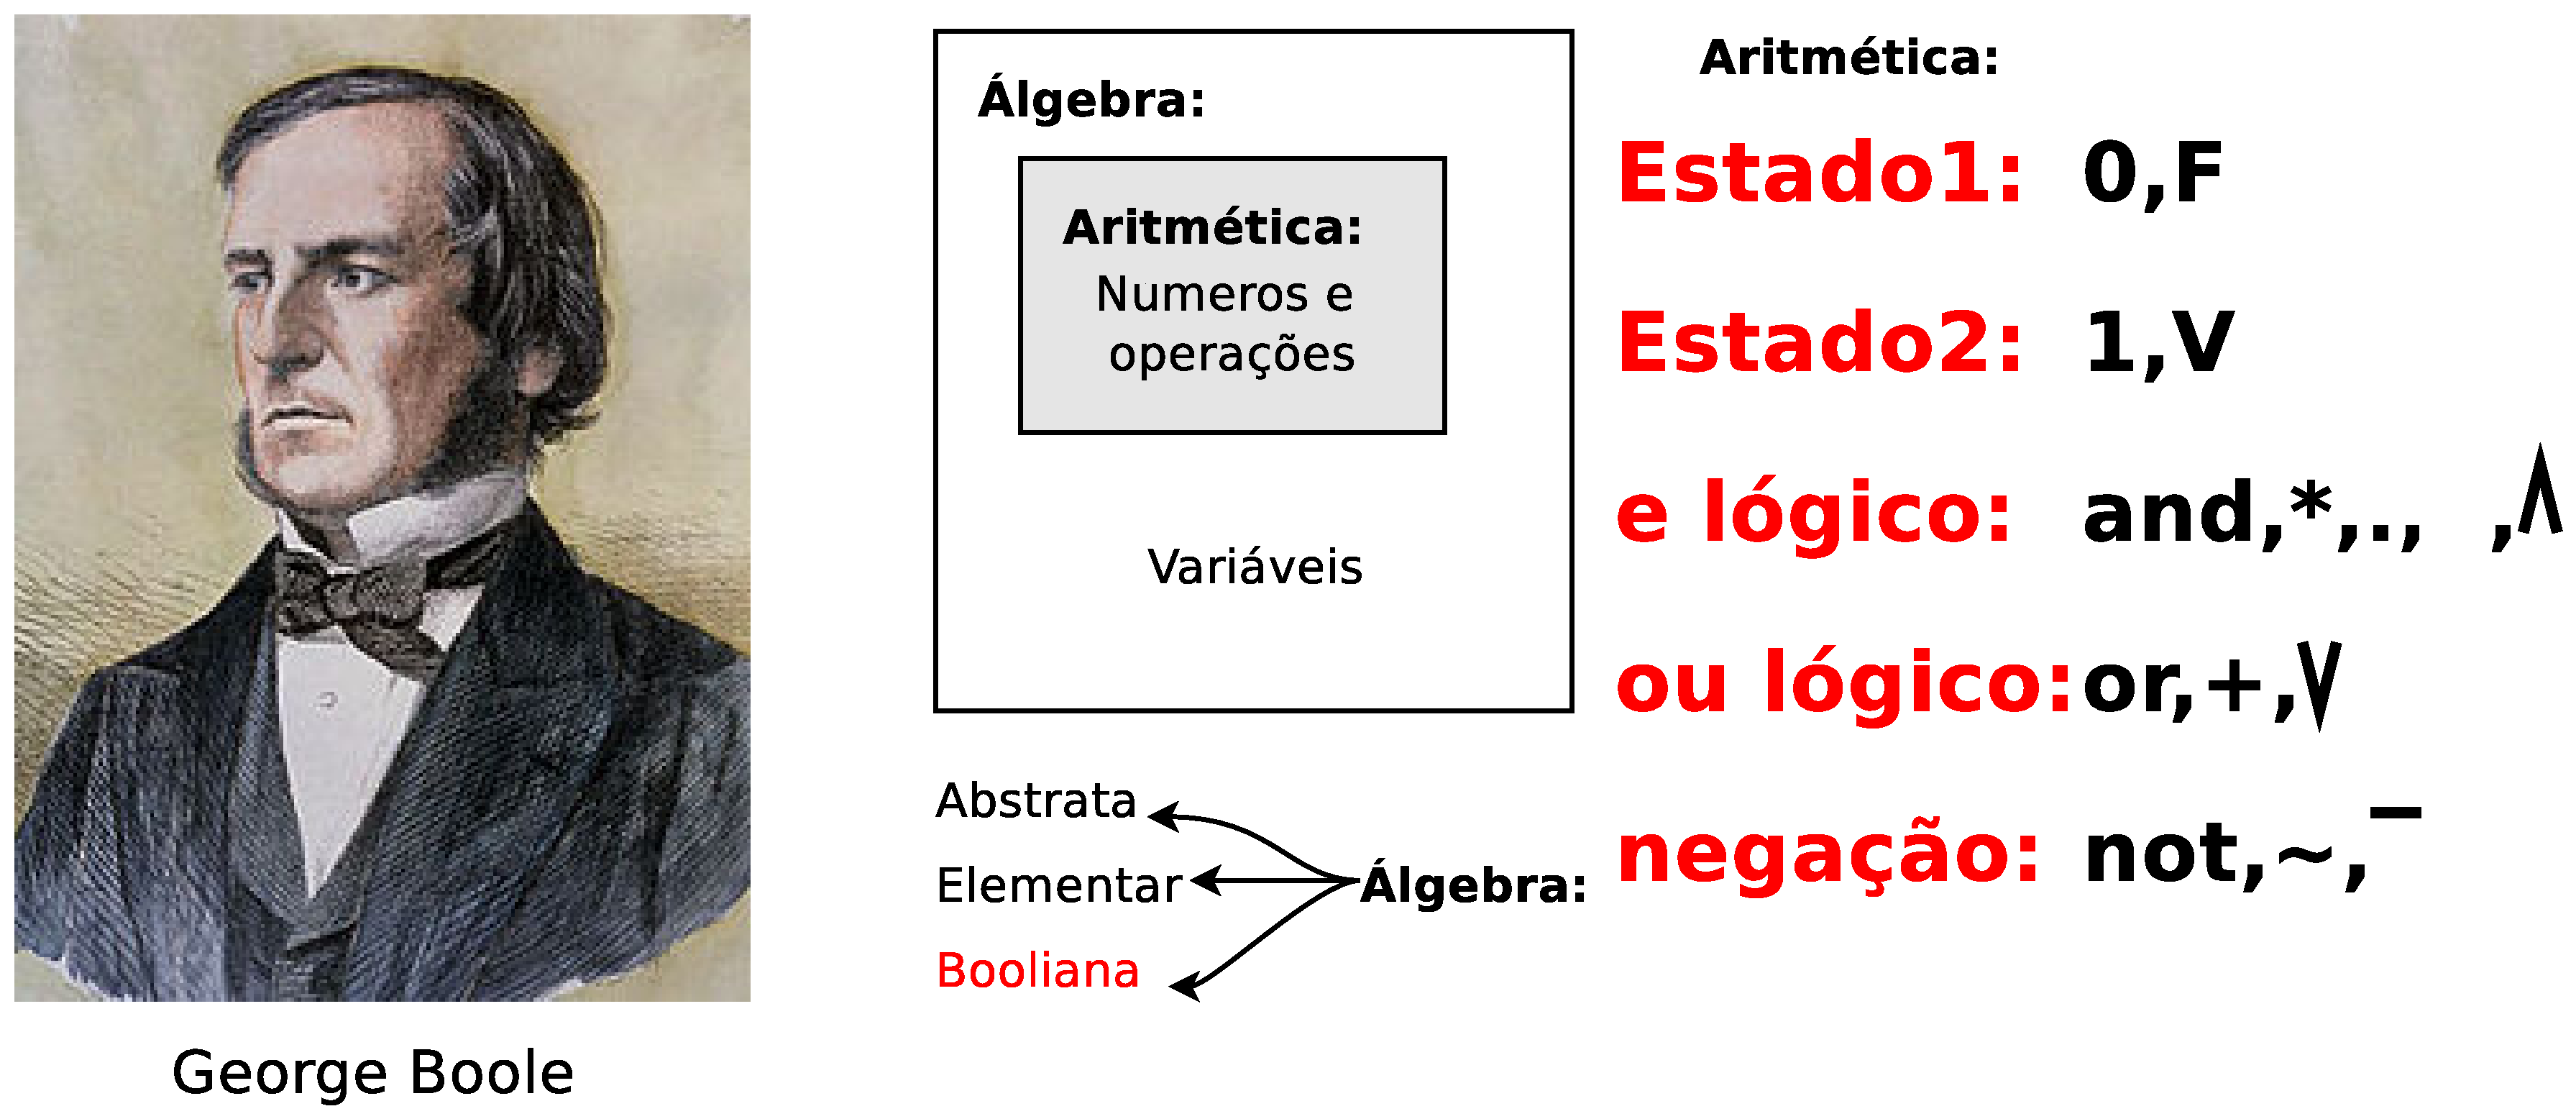
\includegraphics[width=0.99\textwidth]{images/Diagrama1.eps}
\end{center} 
\end{frame}


%%%%%%%%%%%%%%%%%%%%%%%%%%%%%%%%%%%%%%%%%%%%%%%%%%%%%%%%%%%%%%%%%%%%%%%%%%%%%%%%
\begin{frame}{AND}
\begin{center}
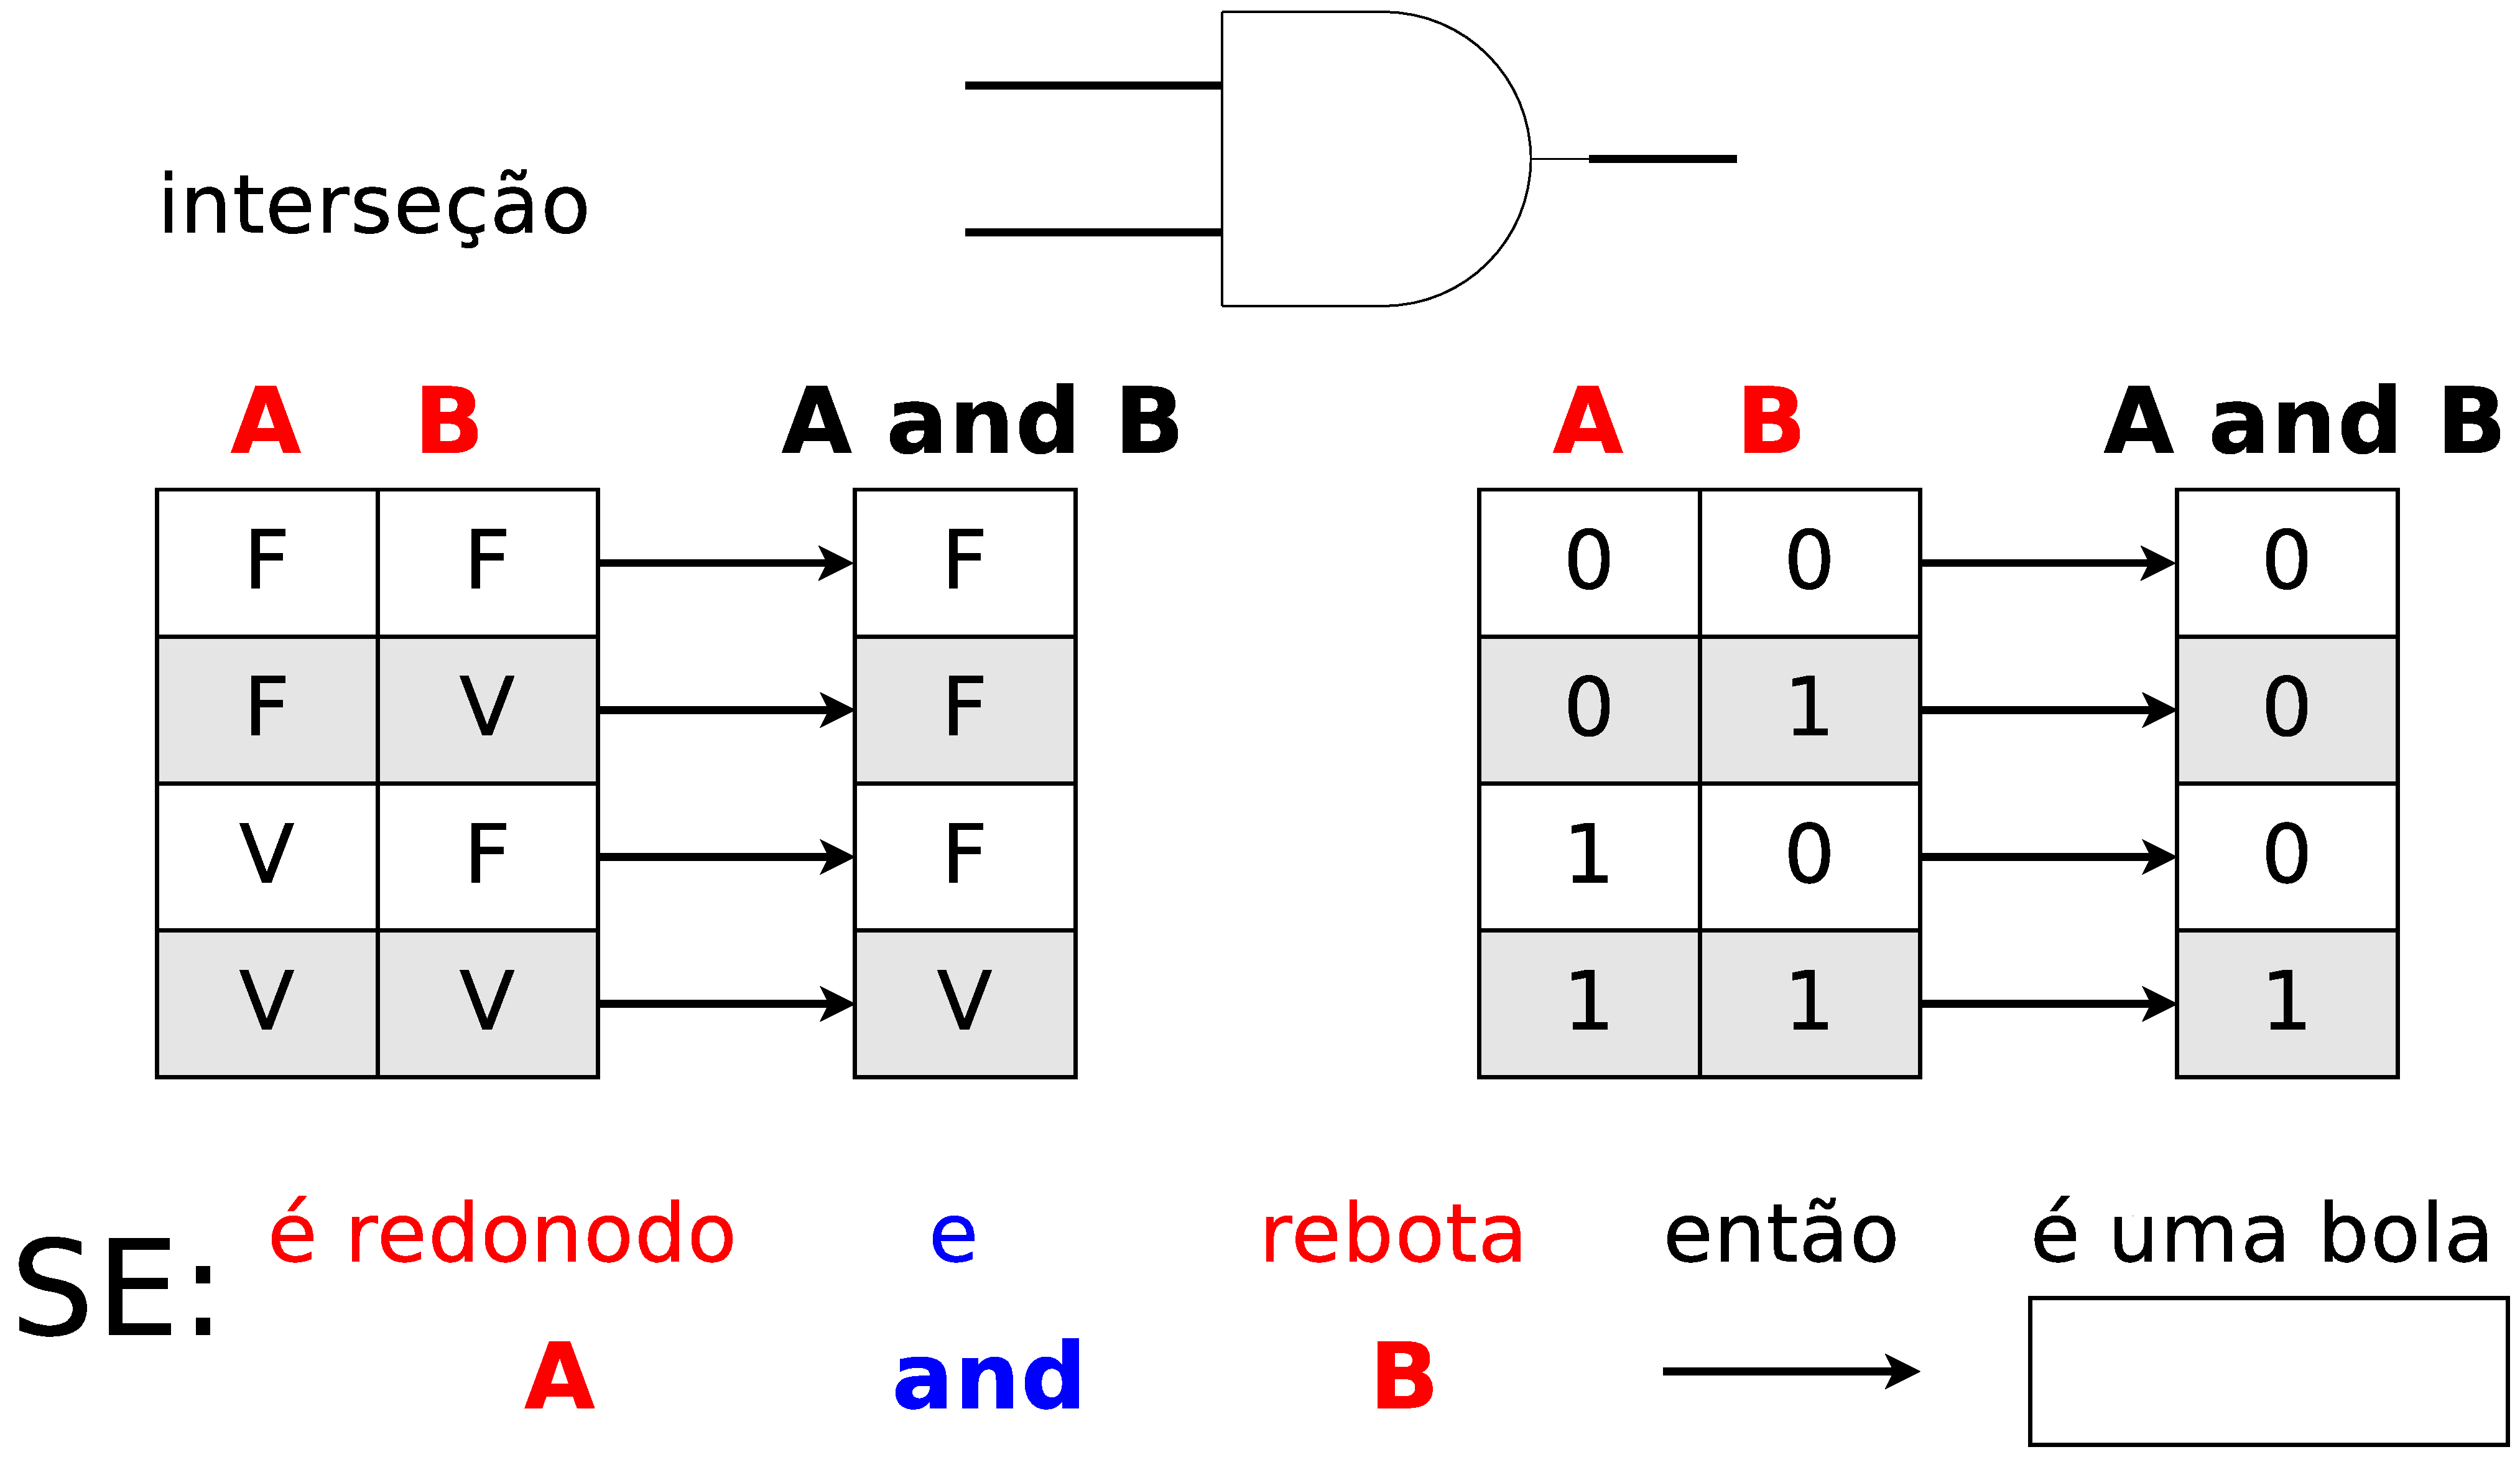
\includegraphics[width=0.99\textwidth]{images/and1.eps}
\end{center} 
\end{frame}


%%%%%%%%%%%%%%%%%%%%%%%%%%%%%%%%%%%%%%%%%%%%%%%%%%%%%%%%%%%%%%%%%%%%%%%%%%%%%%%%
\begin{frame}{OR}
\begin{center}
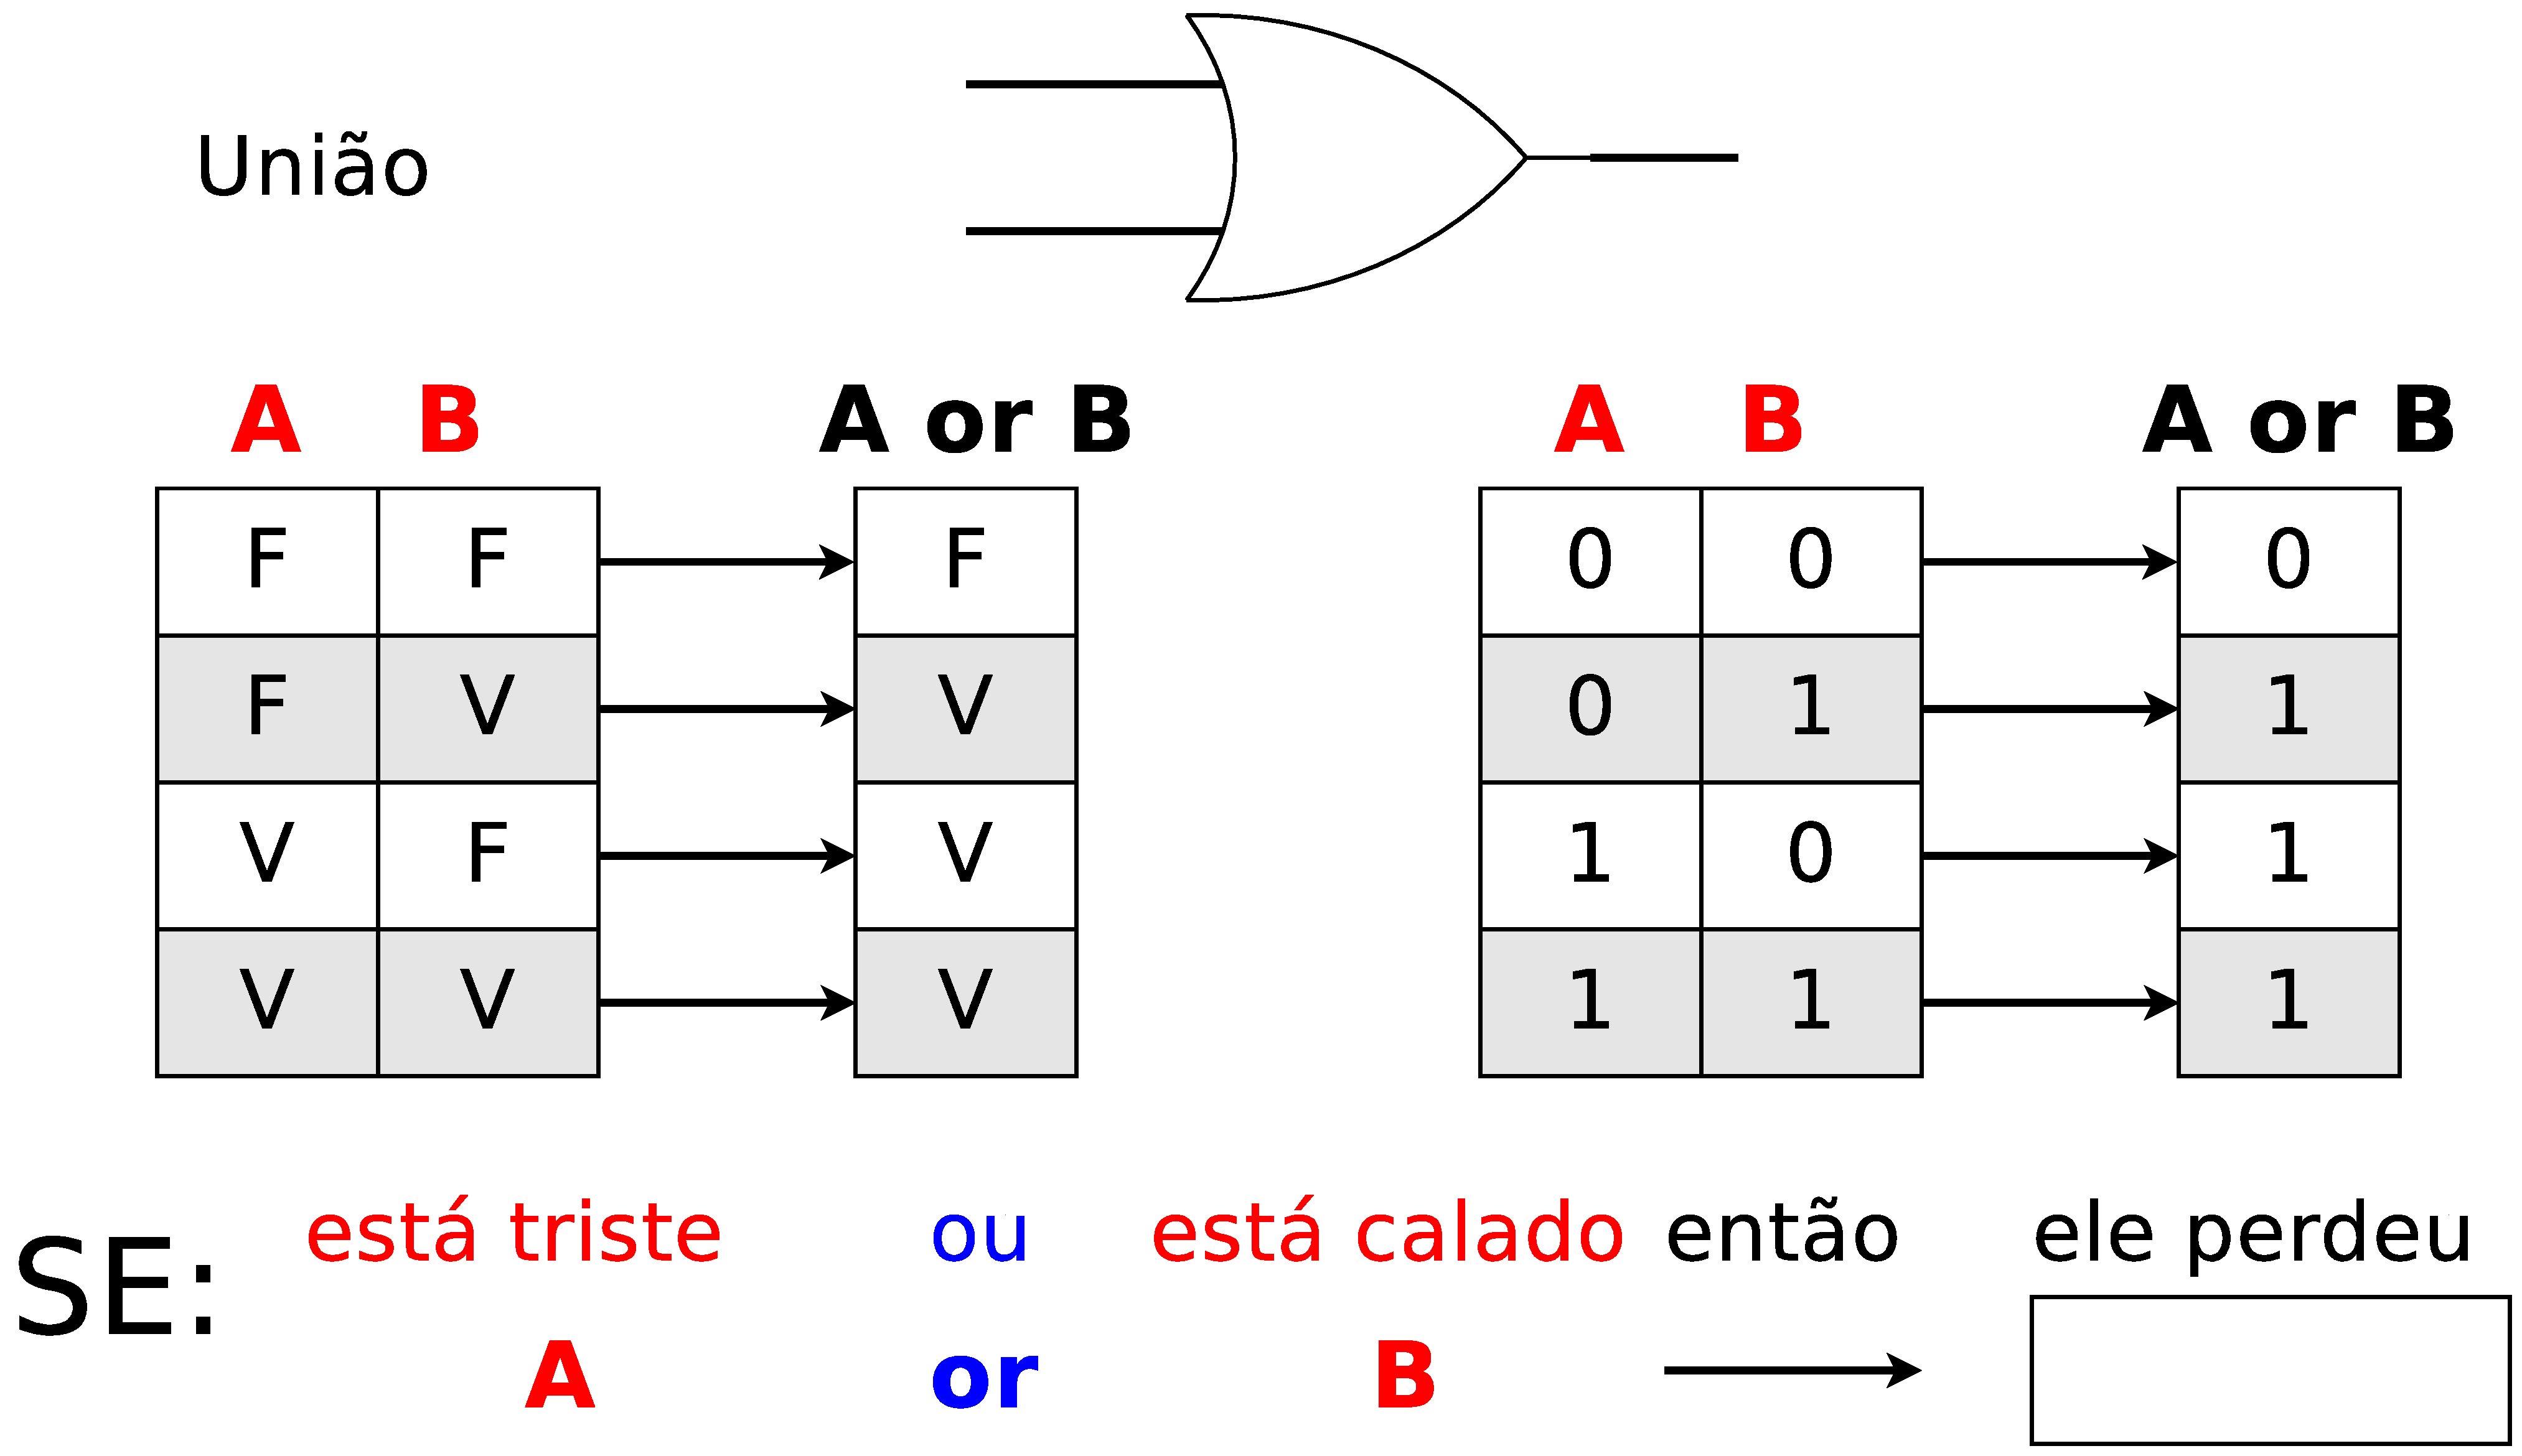
\includegraphics[width=0.99\textwidth]{images/or1.eps}
\end{center} 
\end{frame}


%%%%%%%%%%%%%%%%%%%%%%%%%%%%%%%%%%%%%%%%%%%%%%%%%%%%%%%%%%%%%%%%%%%%%%%%%%%%%%%%
\begin{frame}{NOT}
\begin{center}
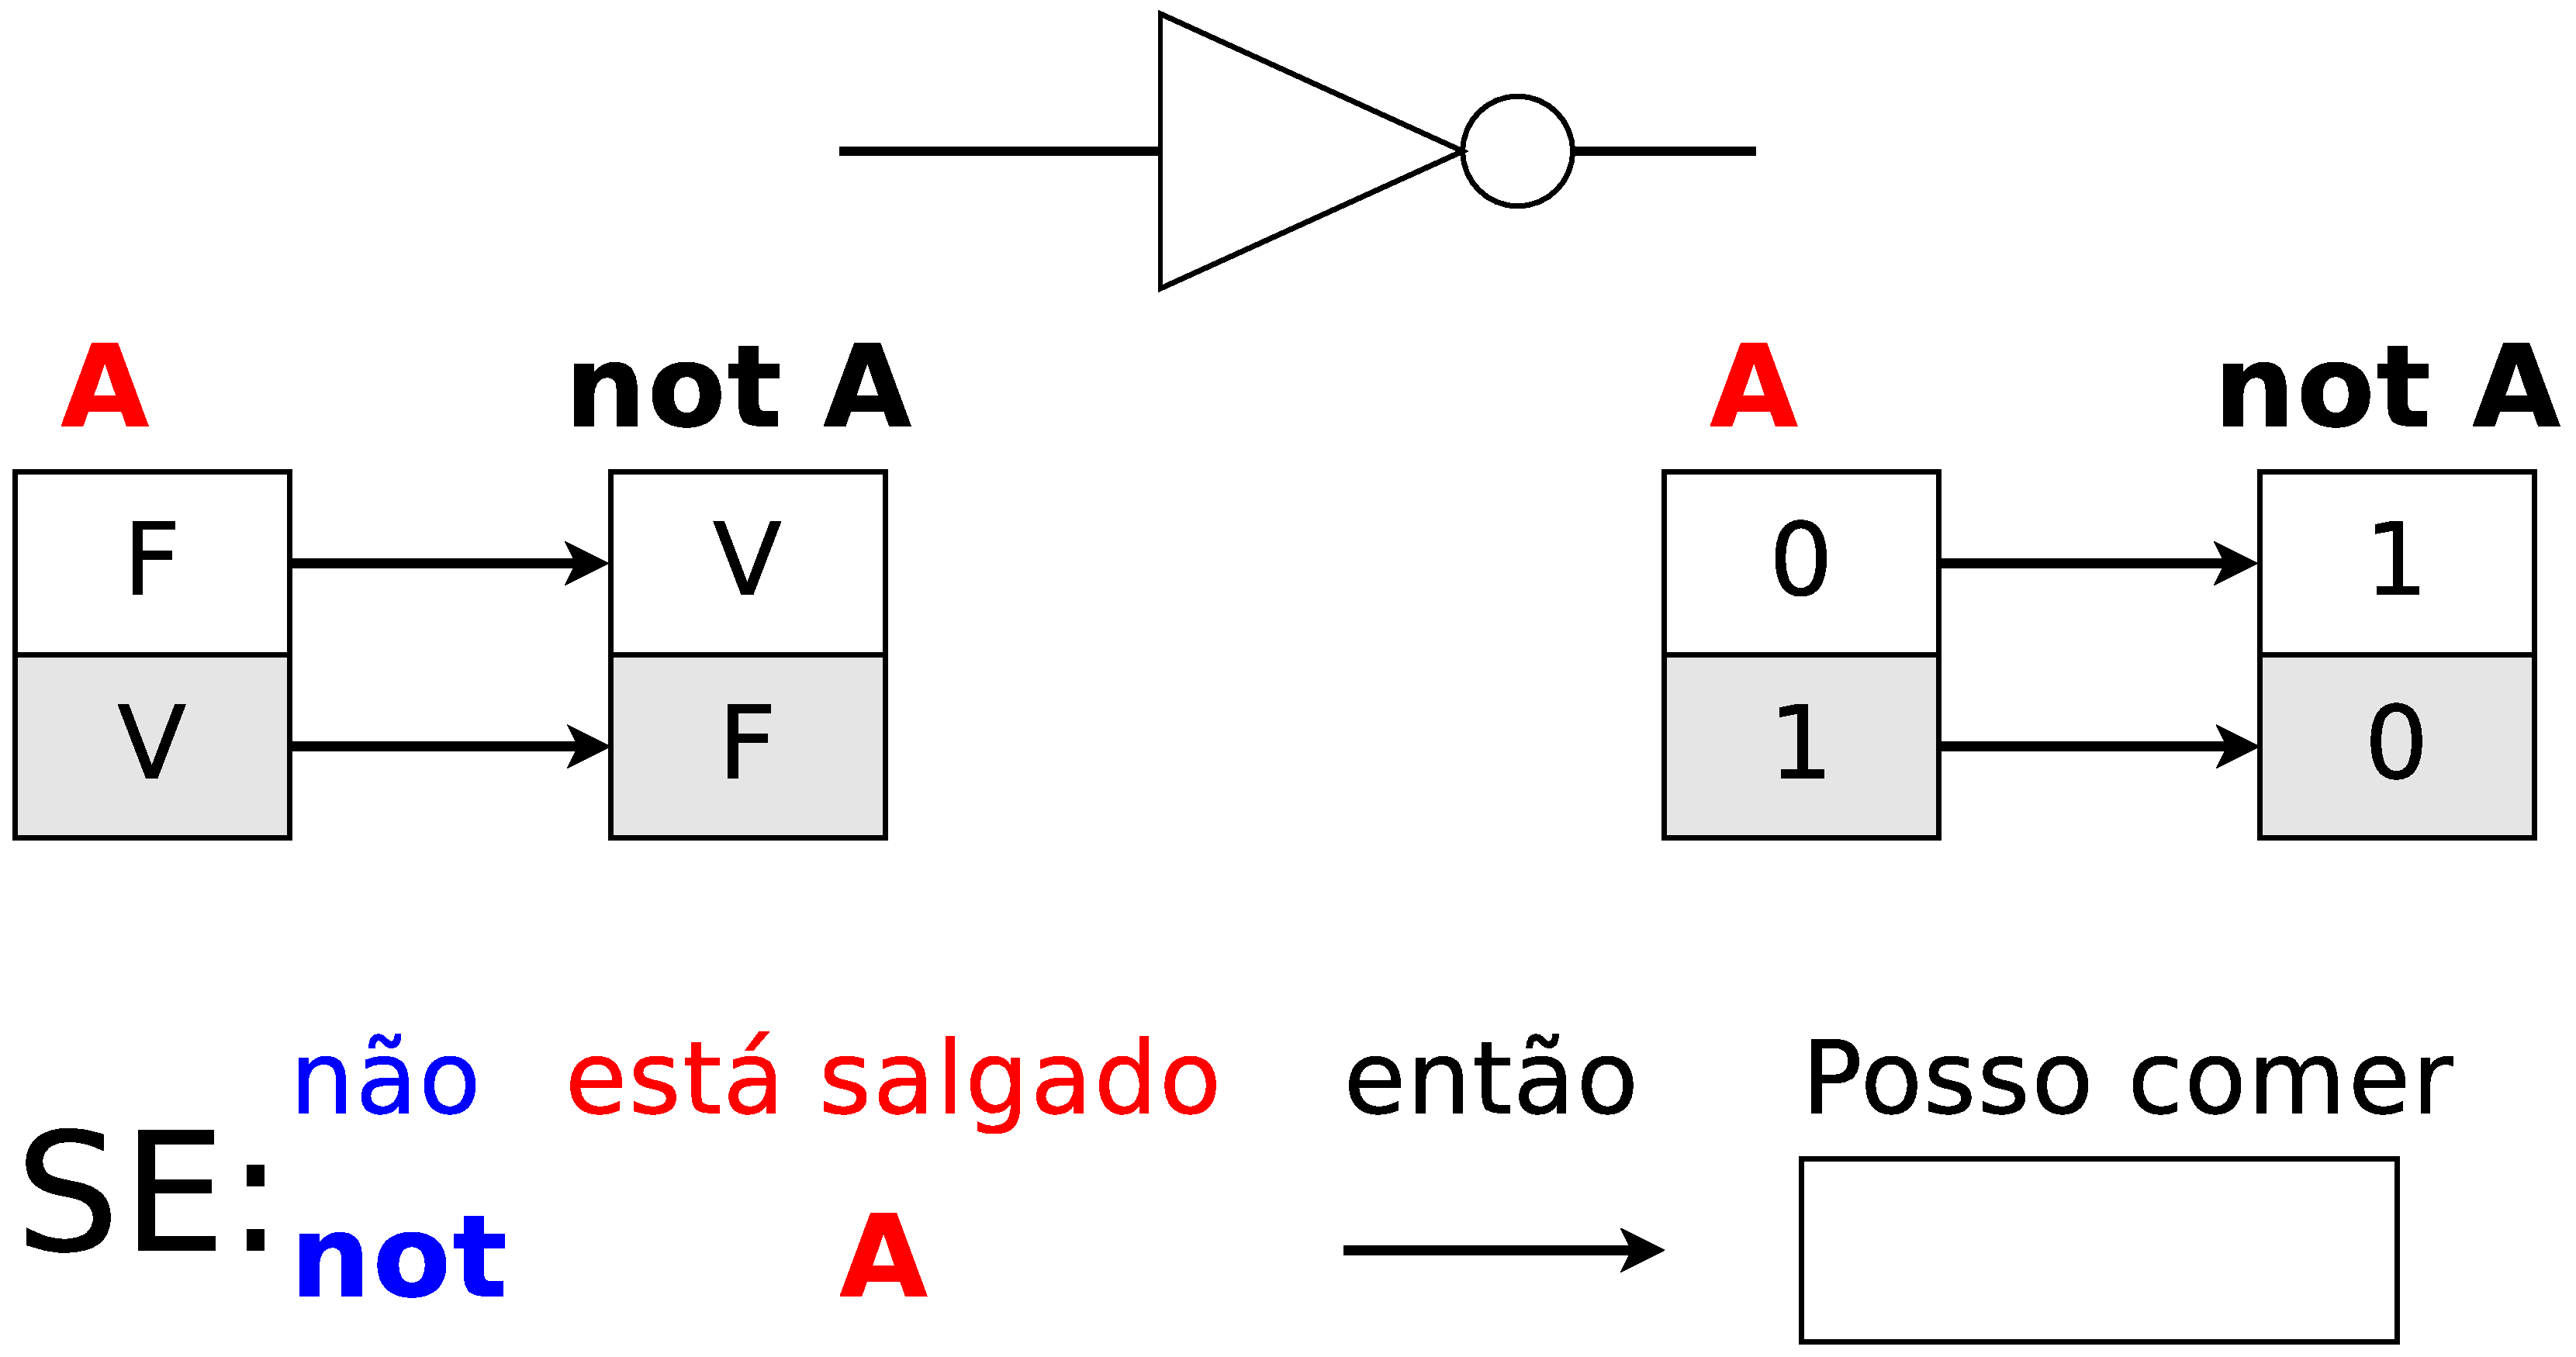
\includegraphics[width=0.99\textwidth]{images/not1.eps}
\end{center} 
\end{frame}

%%%%%%%%%%%%%%%%%%%%%%%%%%%%%%%%%%%%%%%%%%%%%%%%%%%%%%%%%%%%%%%%%%%%%%%%%%%%%%%%
\begin{frame}{Propriedades}
\begin{center}
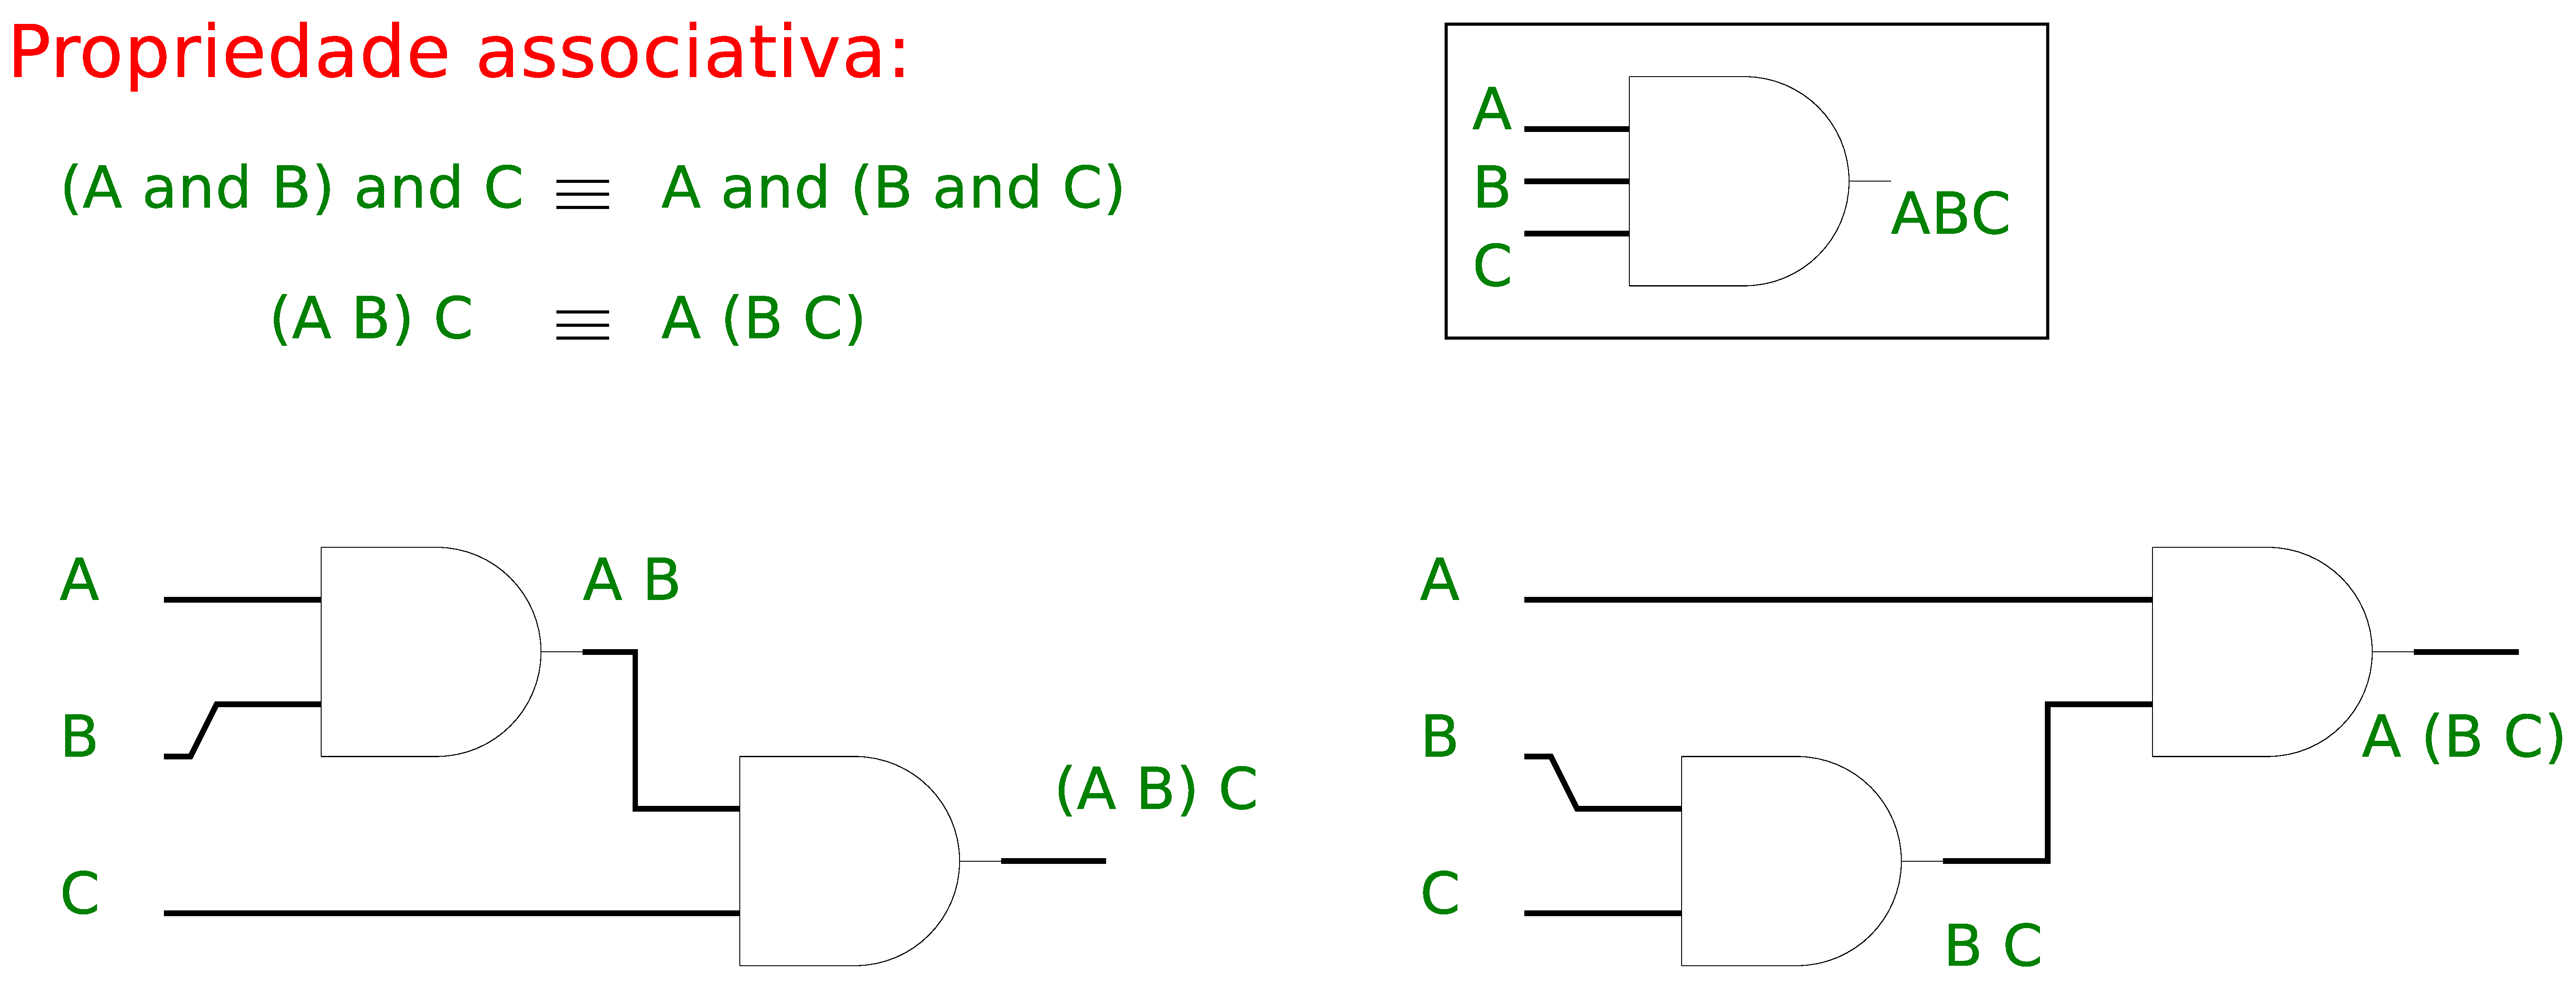
\includegraphics[width=0.99\textwidth]{images/Diagrama2.eps}
\end{center} 
\end{frame}

%%%%%%%%%%%%%%%%%%%%%%%%%%%%%%%%%%%%%%%%%%%%%%%%%%%%%%%%%%%%%%%%%%%%%%%%%%%%%%%%
\begin{frame}{Propriedades}
\begin{center}
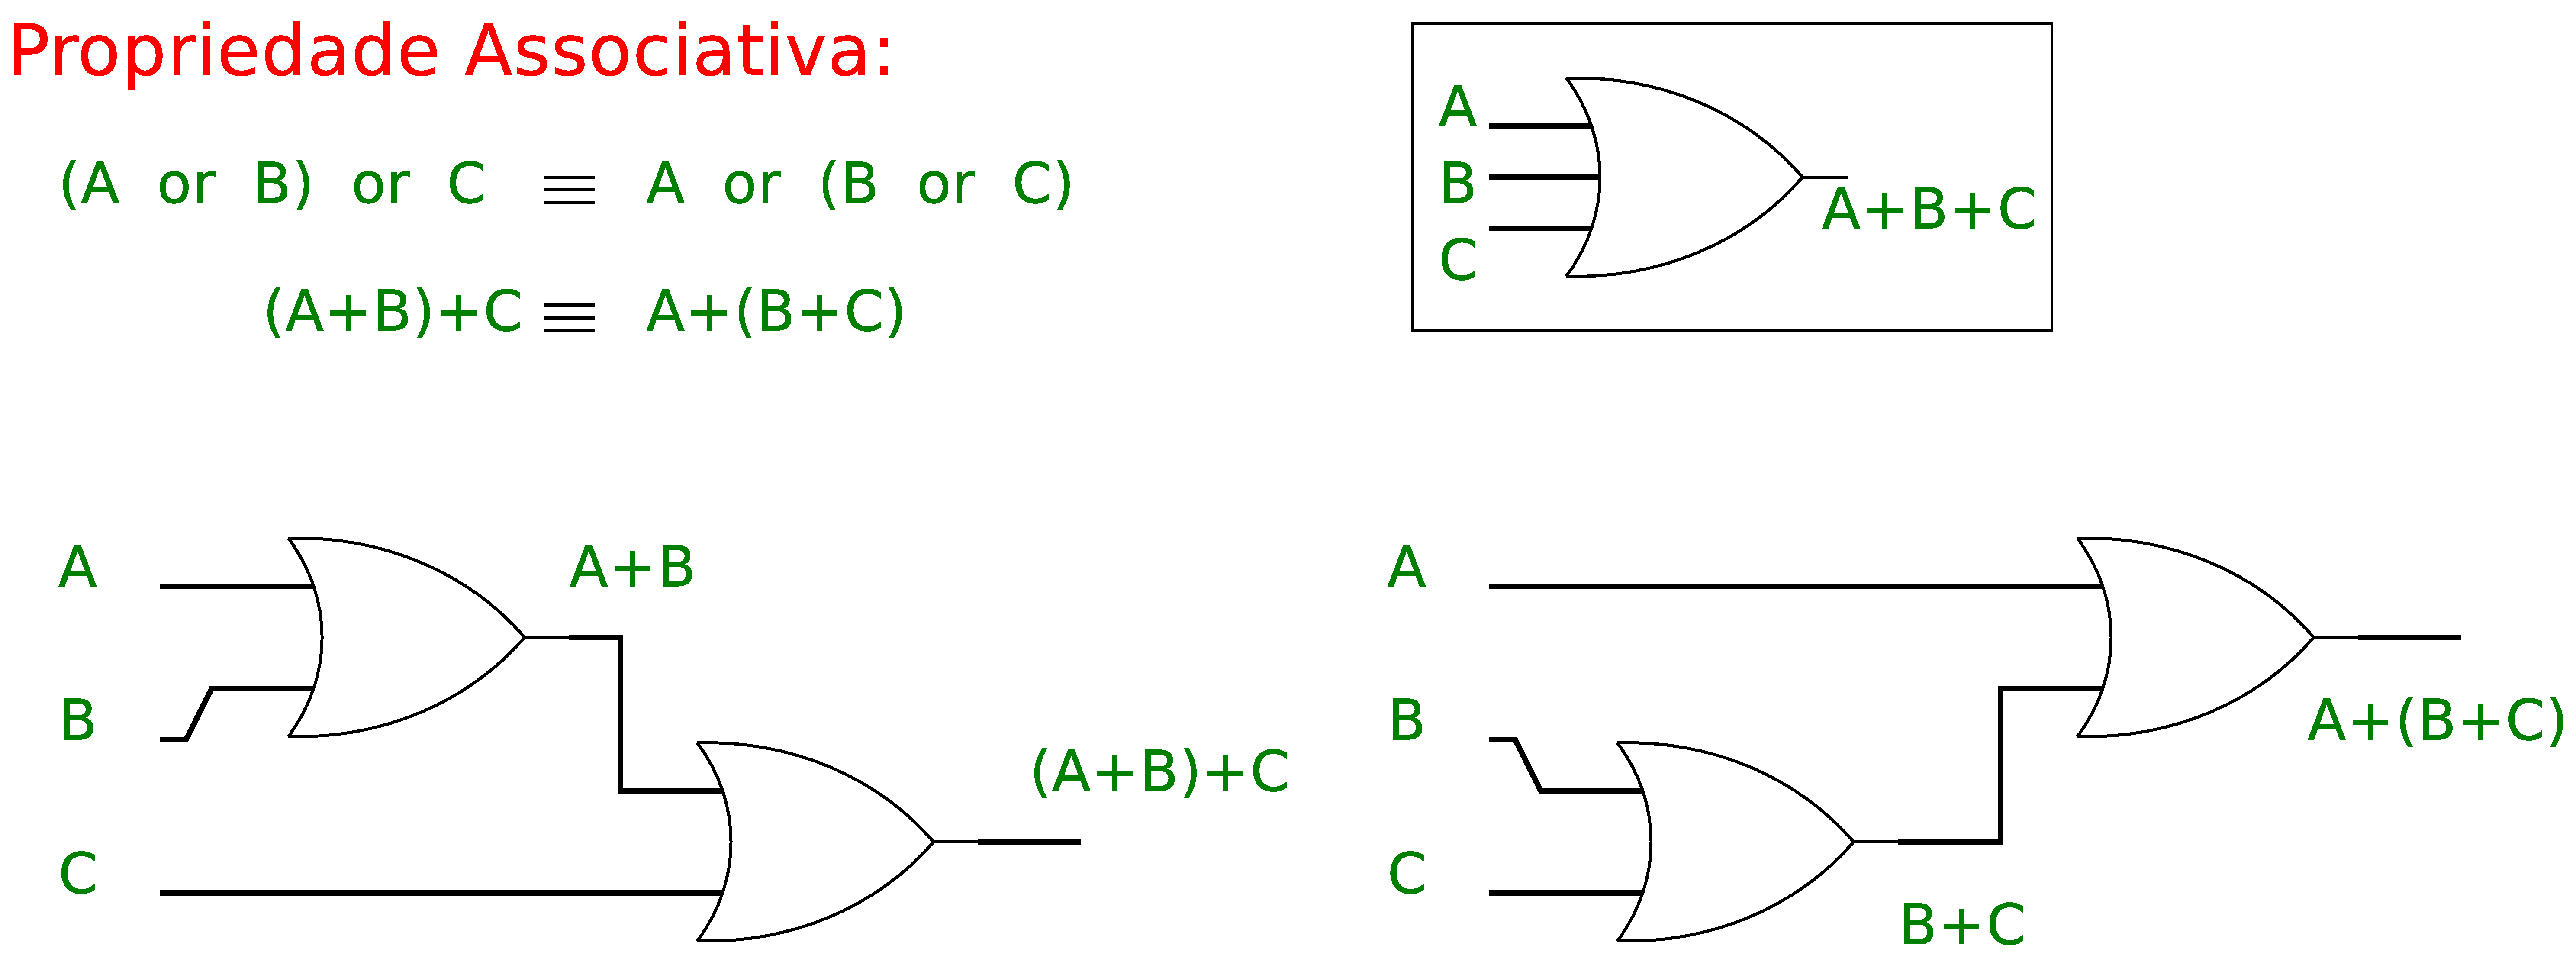
\includegraphics[width=0.99\textwidth]{images/Diagrama2a.eps}
\end{center} 
\end{frame}


%%%%%%%%%%%%%%%%%%%%%%%%%%%%%%%%%%%%%%%%%%%%%%%%%%%%%%%%%%%%%%%%%%%%%%%%%%%%%%%%
\begin{frame}{Propriedades}
\begin{center}
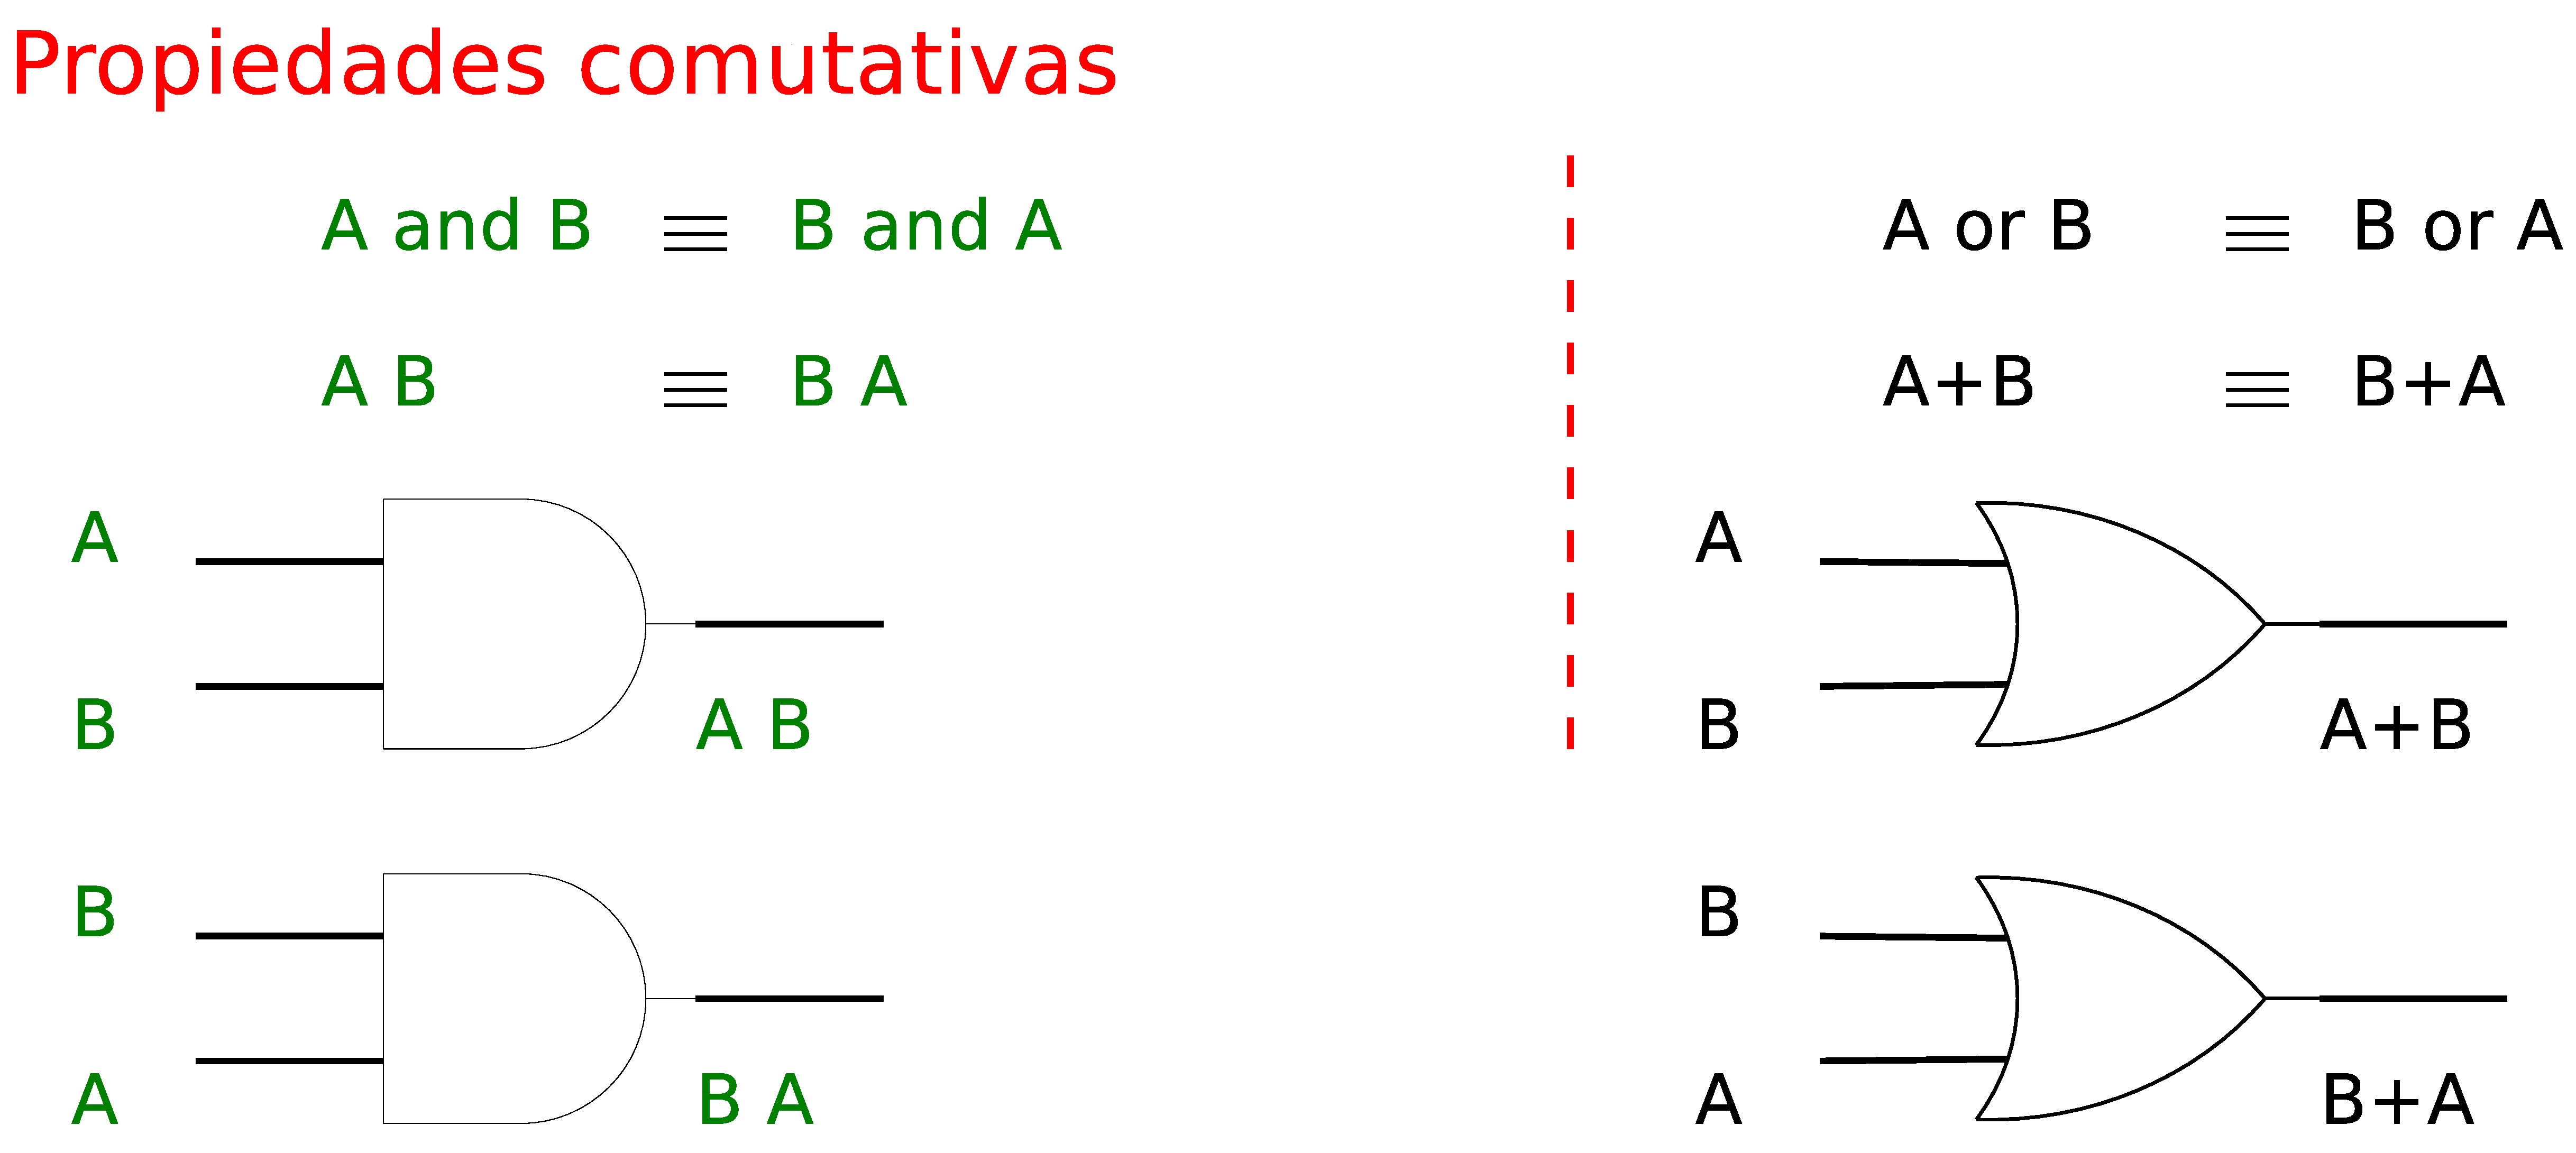
\includegraphics[width=0.99\textwidth]{images/comutativa.eps}
\end{center} 
\end{frame}

%%%%%%%%%%%%%%%%%%%%%%%%%%%%%%%%%%%%%%%%%%%%%%%%%%%%%%%%%%%%%%%%%%%%%%%%%%%%%%%%
\begin{frame}{Propriedades}
\begin{center}
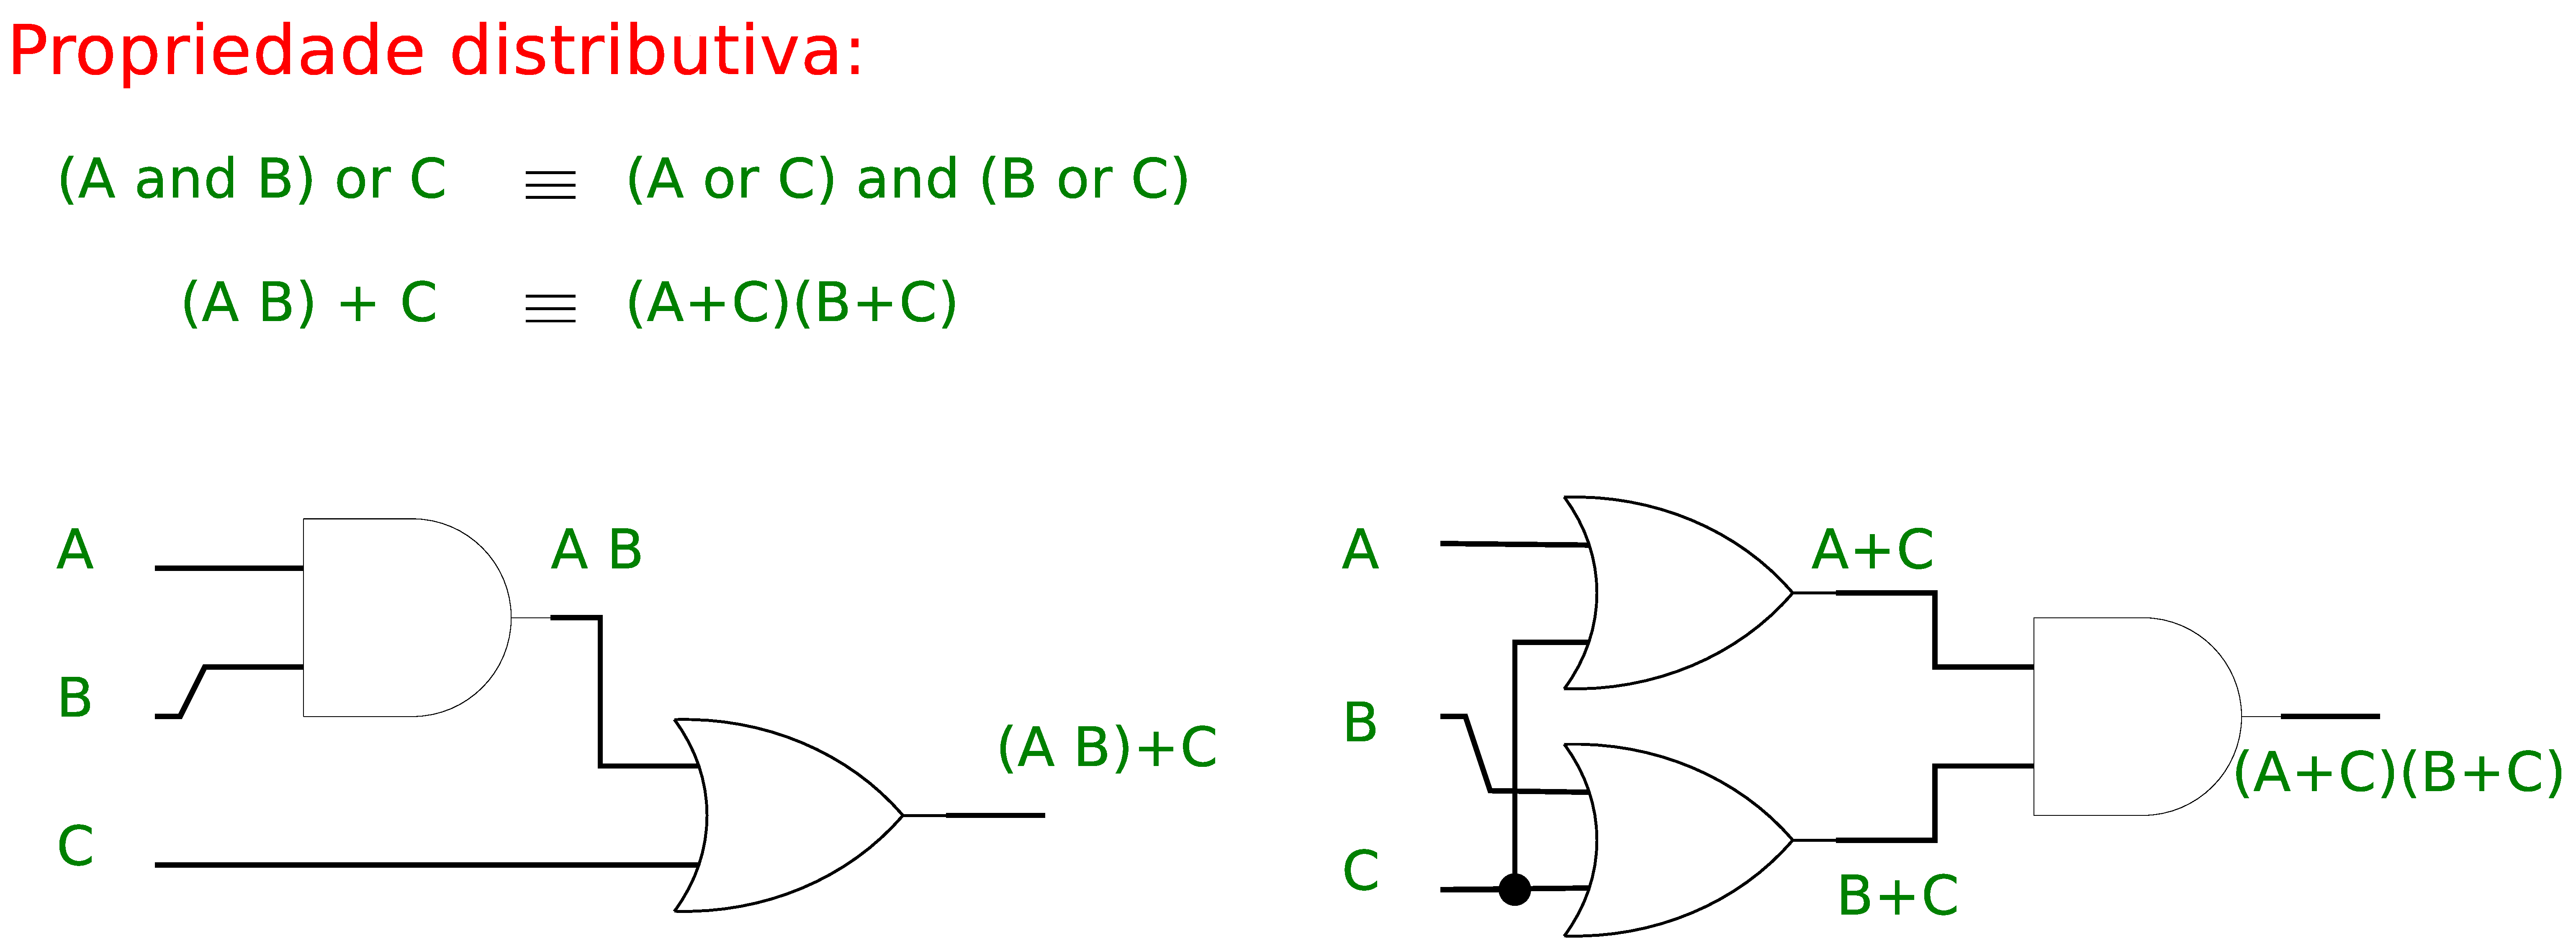
\includegraphics[width=0.99\textwidth]{images/distributiva.eps}
\end{center} 
\end{frame}

%%%%%%%%%%%%%%%%%%%%%%%%%%%%%%%%%%%%%%%%%%%%%%%%%%%%%%%%%%%%%%%%%%%%%%%%%%%%%%%%
\begin{frame}{Propriedades}
\begin{center}
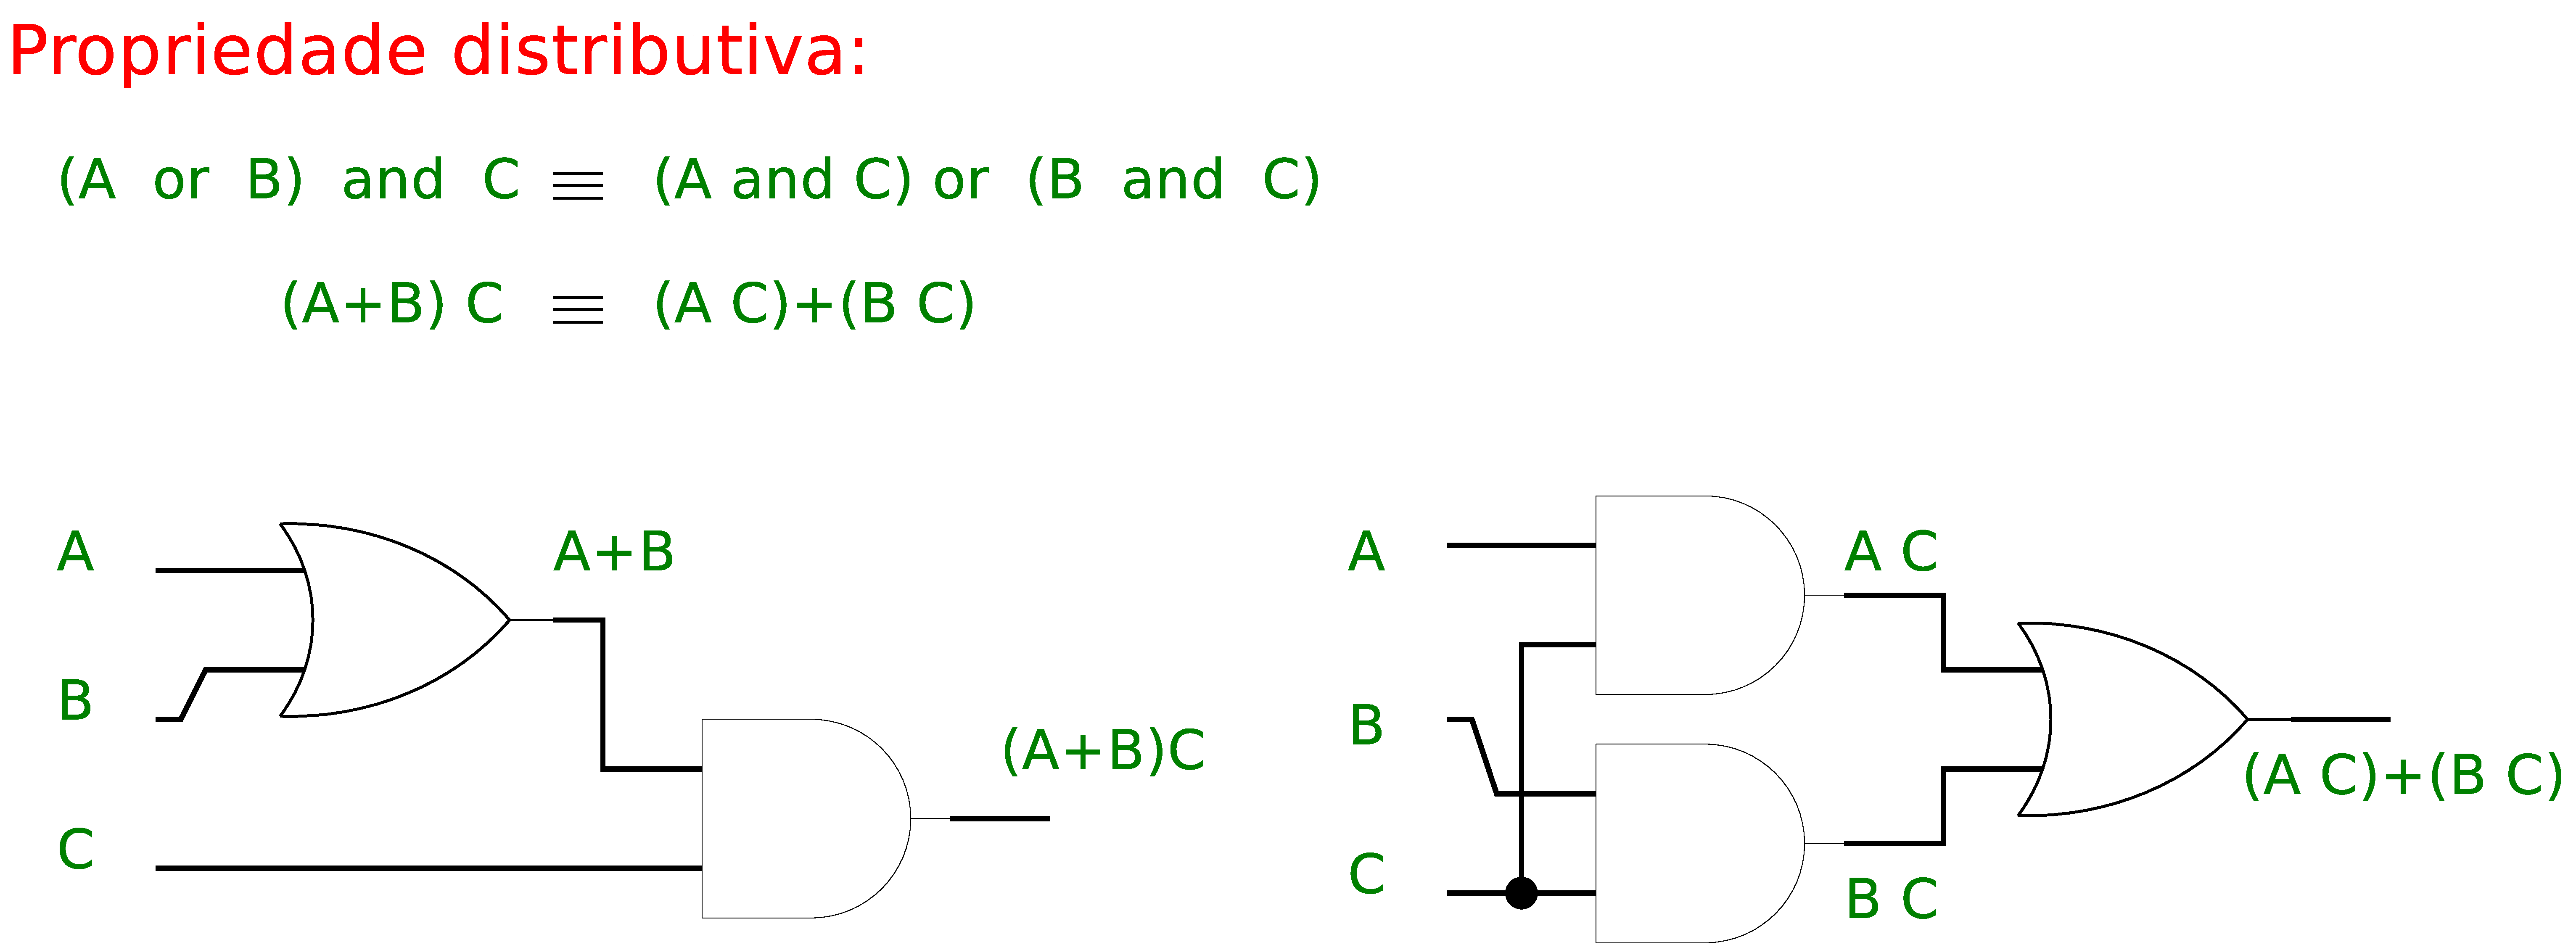
\includegraphics[width=0.99\textwidth]{images/distributivab.eps}
\end{center} 
\end{frame}

%%%%%%%%%%%%%%%%%%%%%%%%%%%%%%%%%%%%%%%%%%%%%%%%%%%%%%%%%%%%%%%%%%%%%%%%%%%%%%%%
\begin{frame}{Propriedades}
\begin{center}
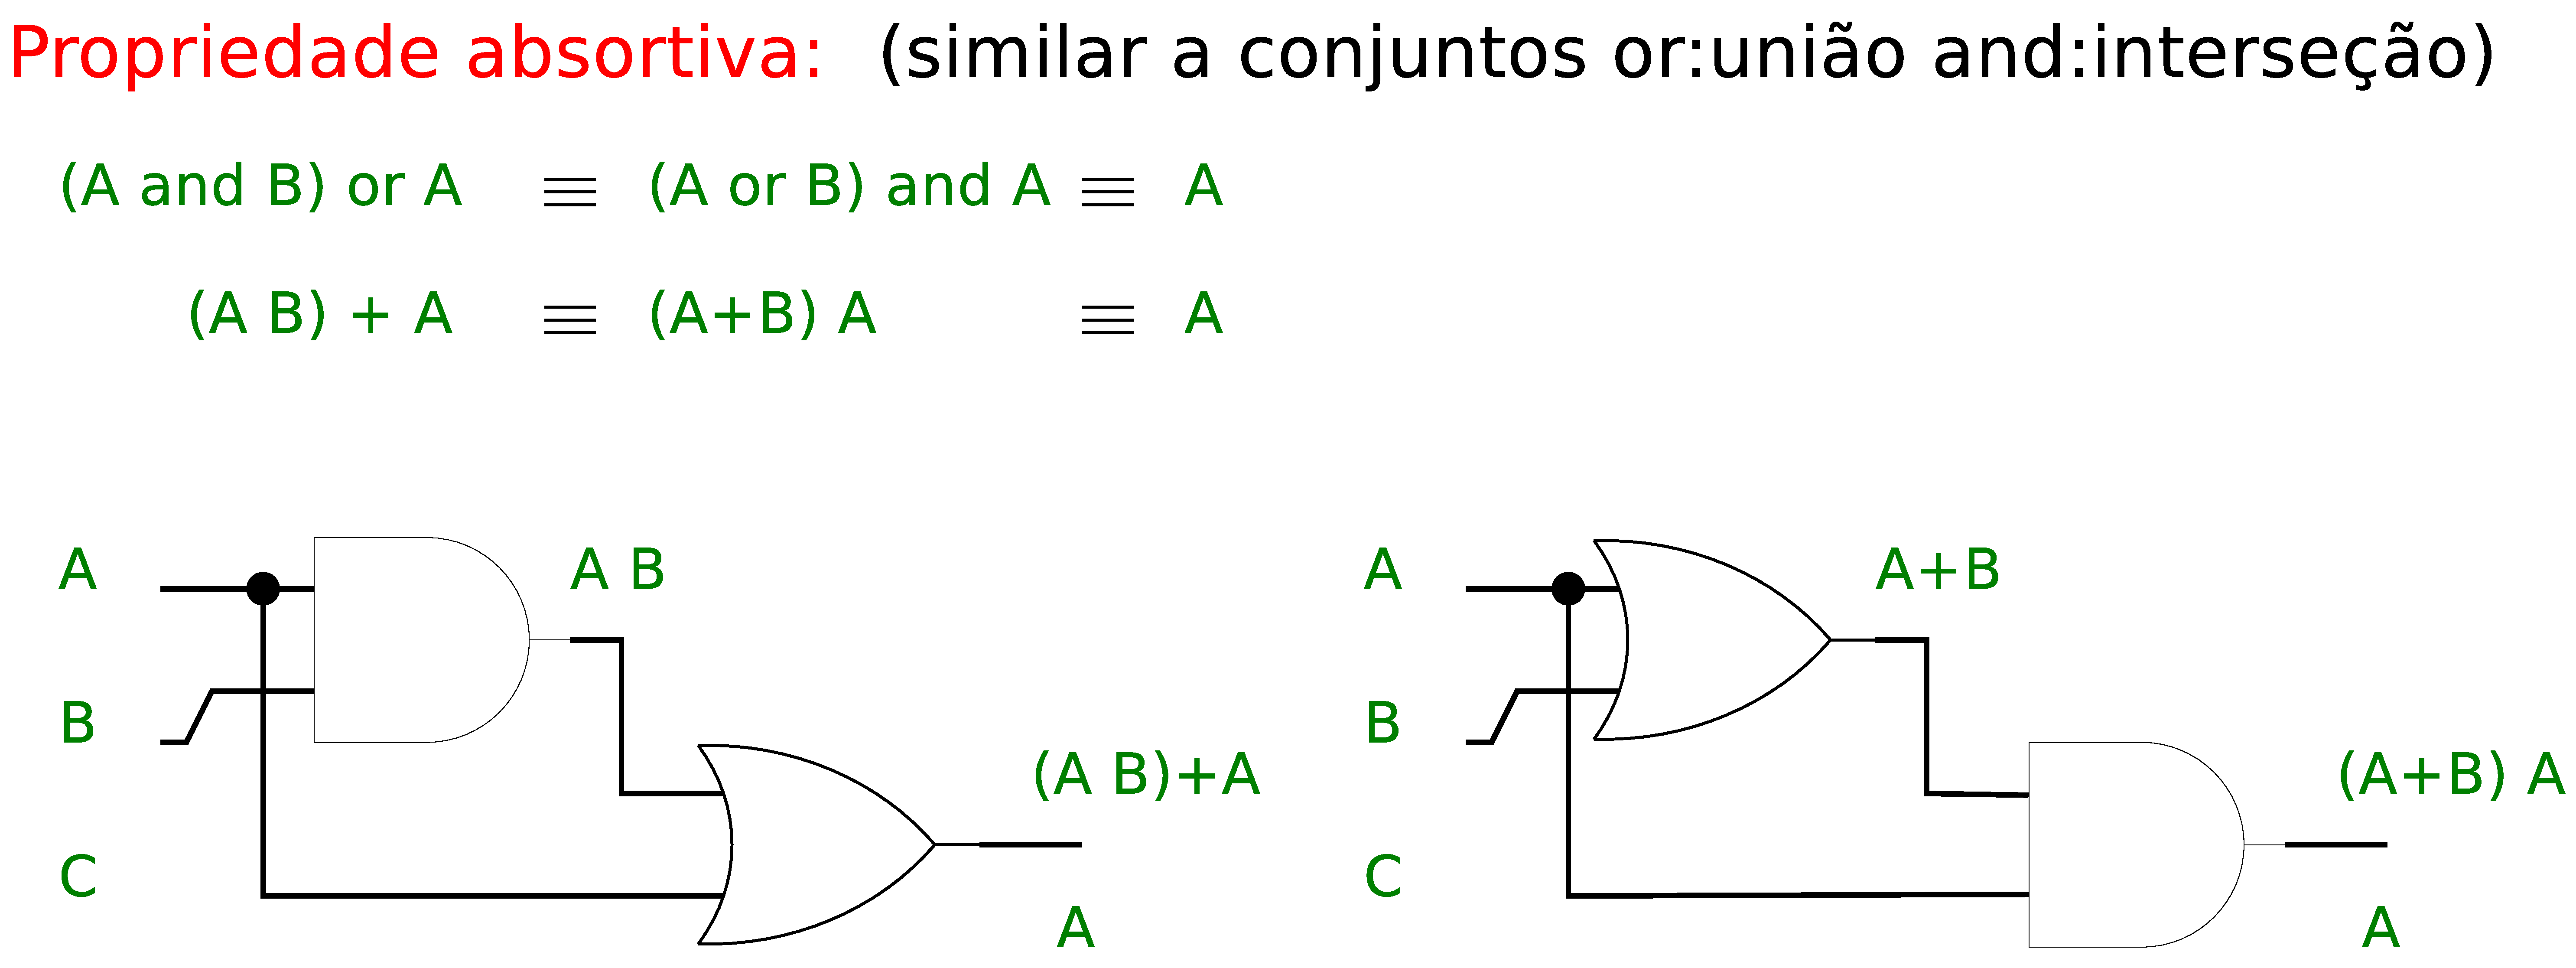
\includegraphics[width=0.99\textwidth]{images/absortivas.eps}
\end{center} 
\end{frame}

%%%%%%%%%%%%%%%%%%%%%%%%%%%%%%%%%%%%%%%%%%%%%%%%%%%%%%%%%%%%%%%%%%%%%%%%%%%%%%%%
\begin{frame}{Propriedades}
\begin{center}
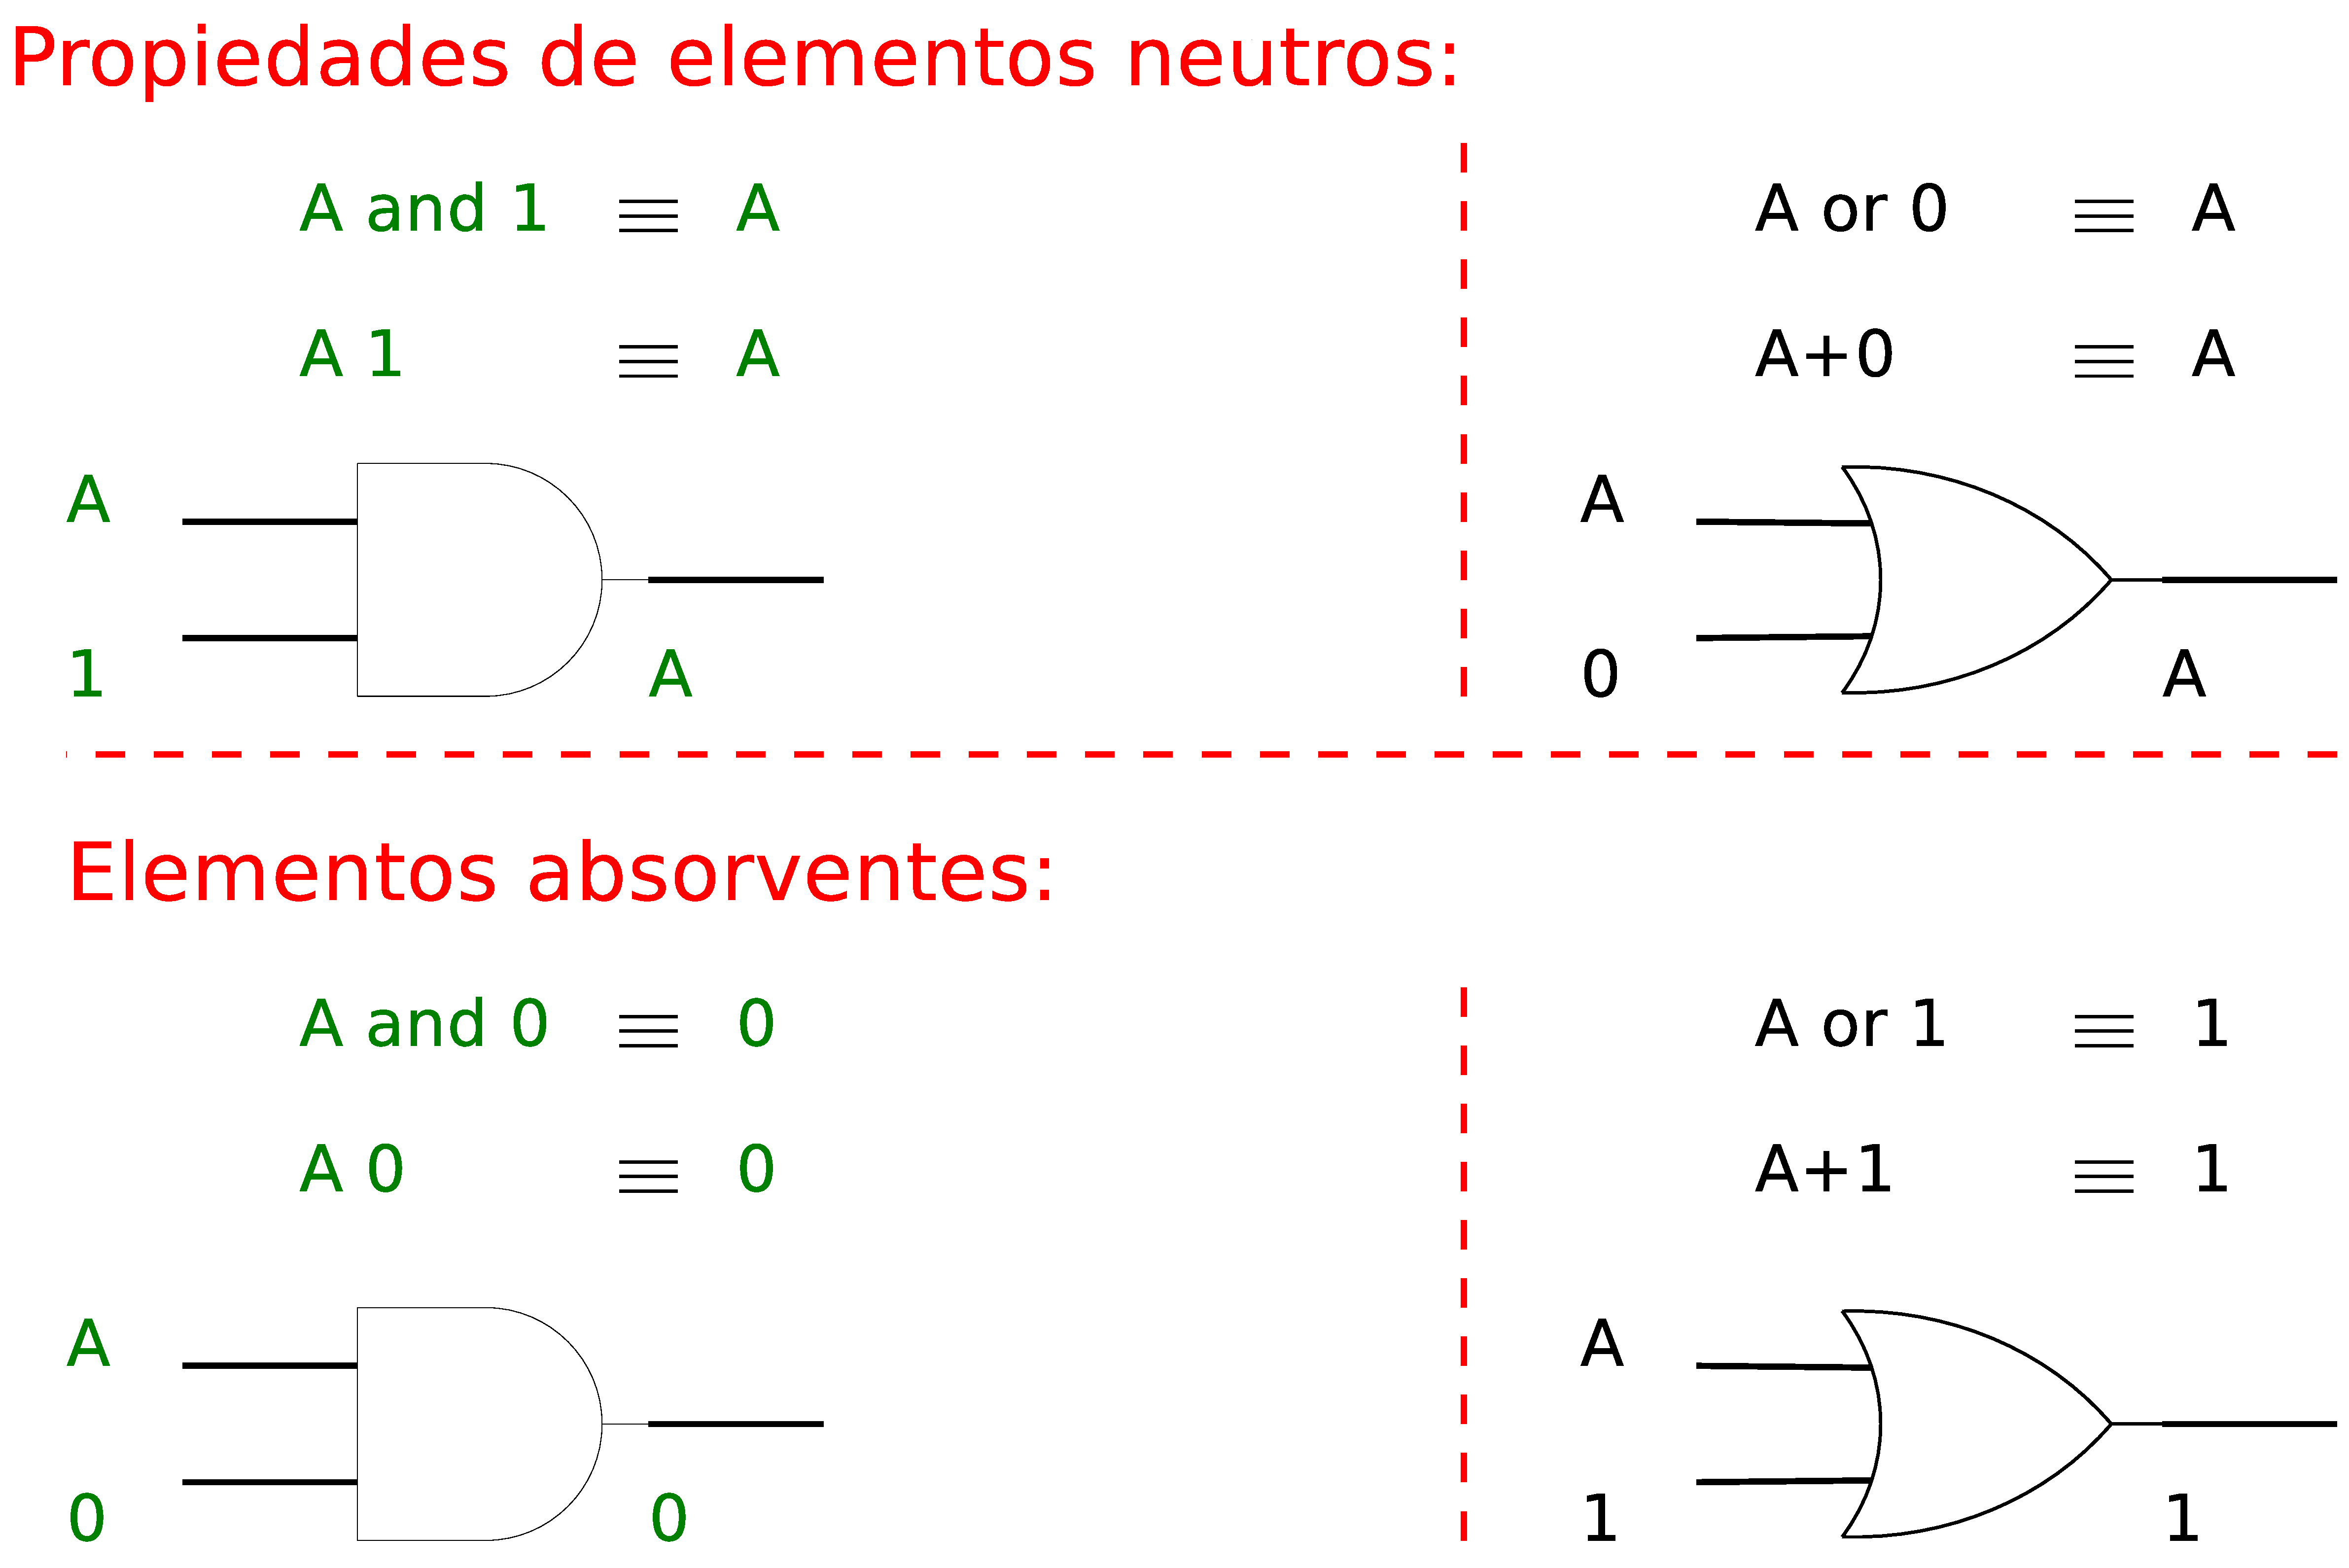
\includegraphics[width=0.99\textwidth]{images/neutro.eps}
\end{center} 
\end{frame}

%%%%%%%%%%%%%%%%%%%%%%%%%%%%%%%%%%%%%%%%%%%%%%%%%%%%%%%%%%%%%%%%%%%%%%%%%%%%%%%%
\begin{frame}{Propriedades}
\begin{center}
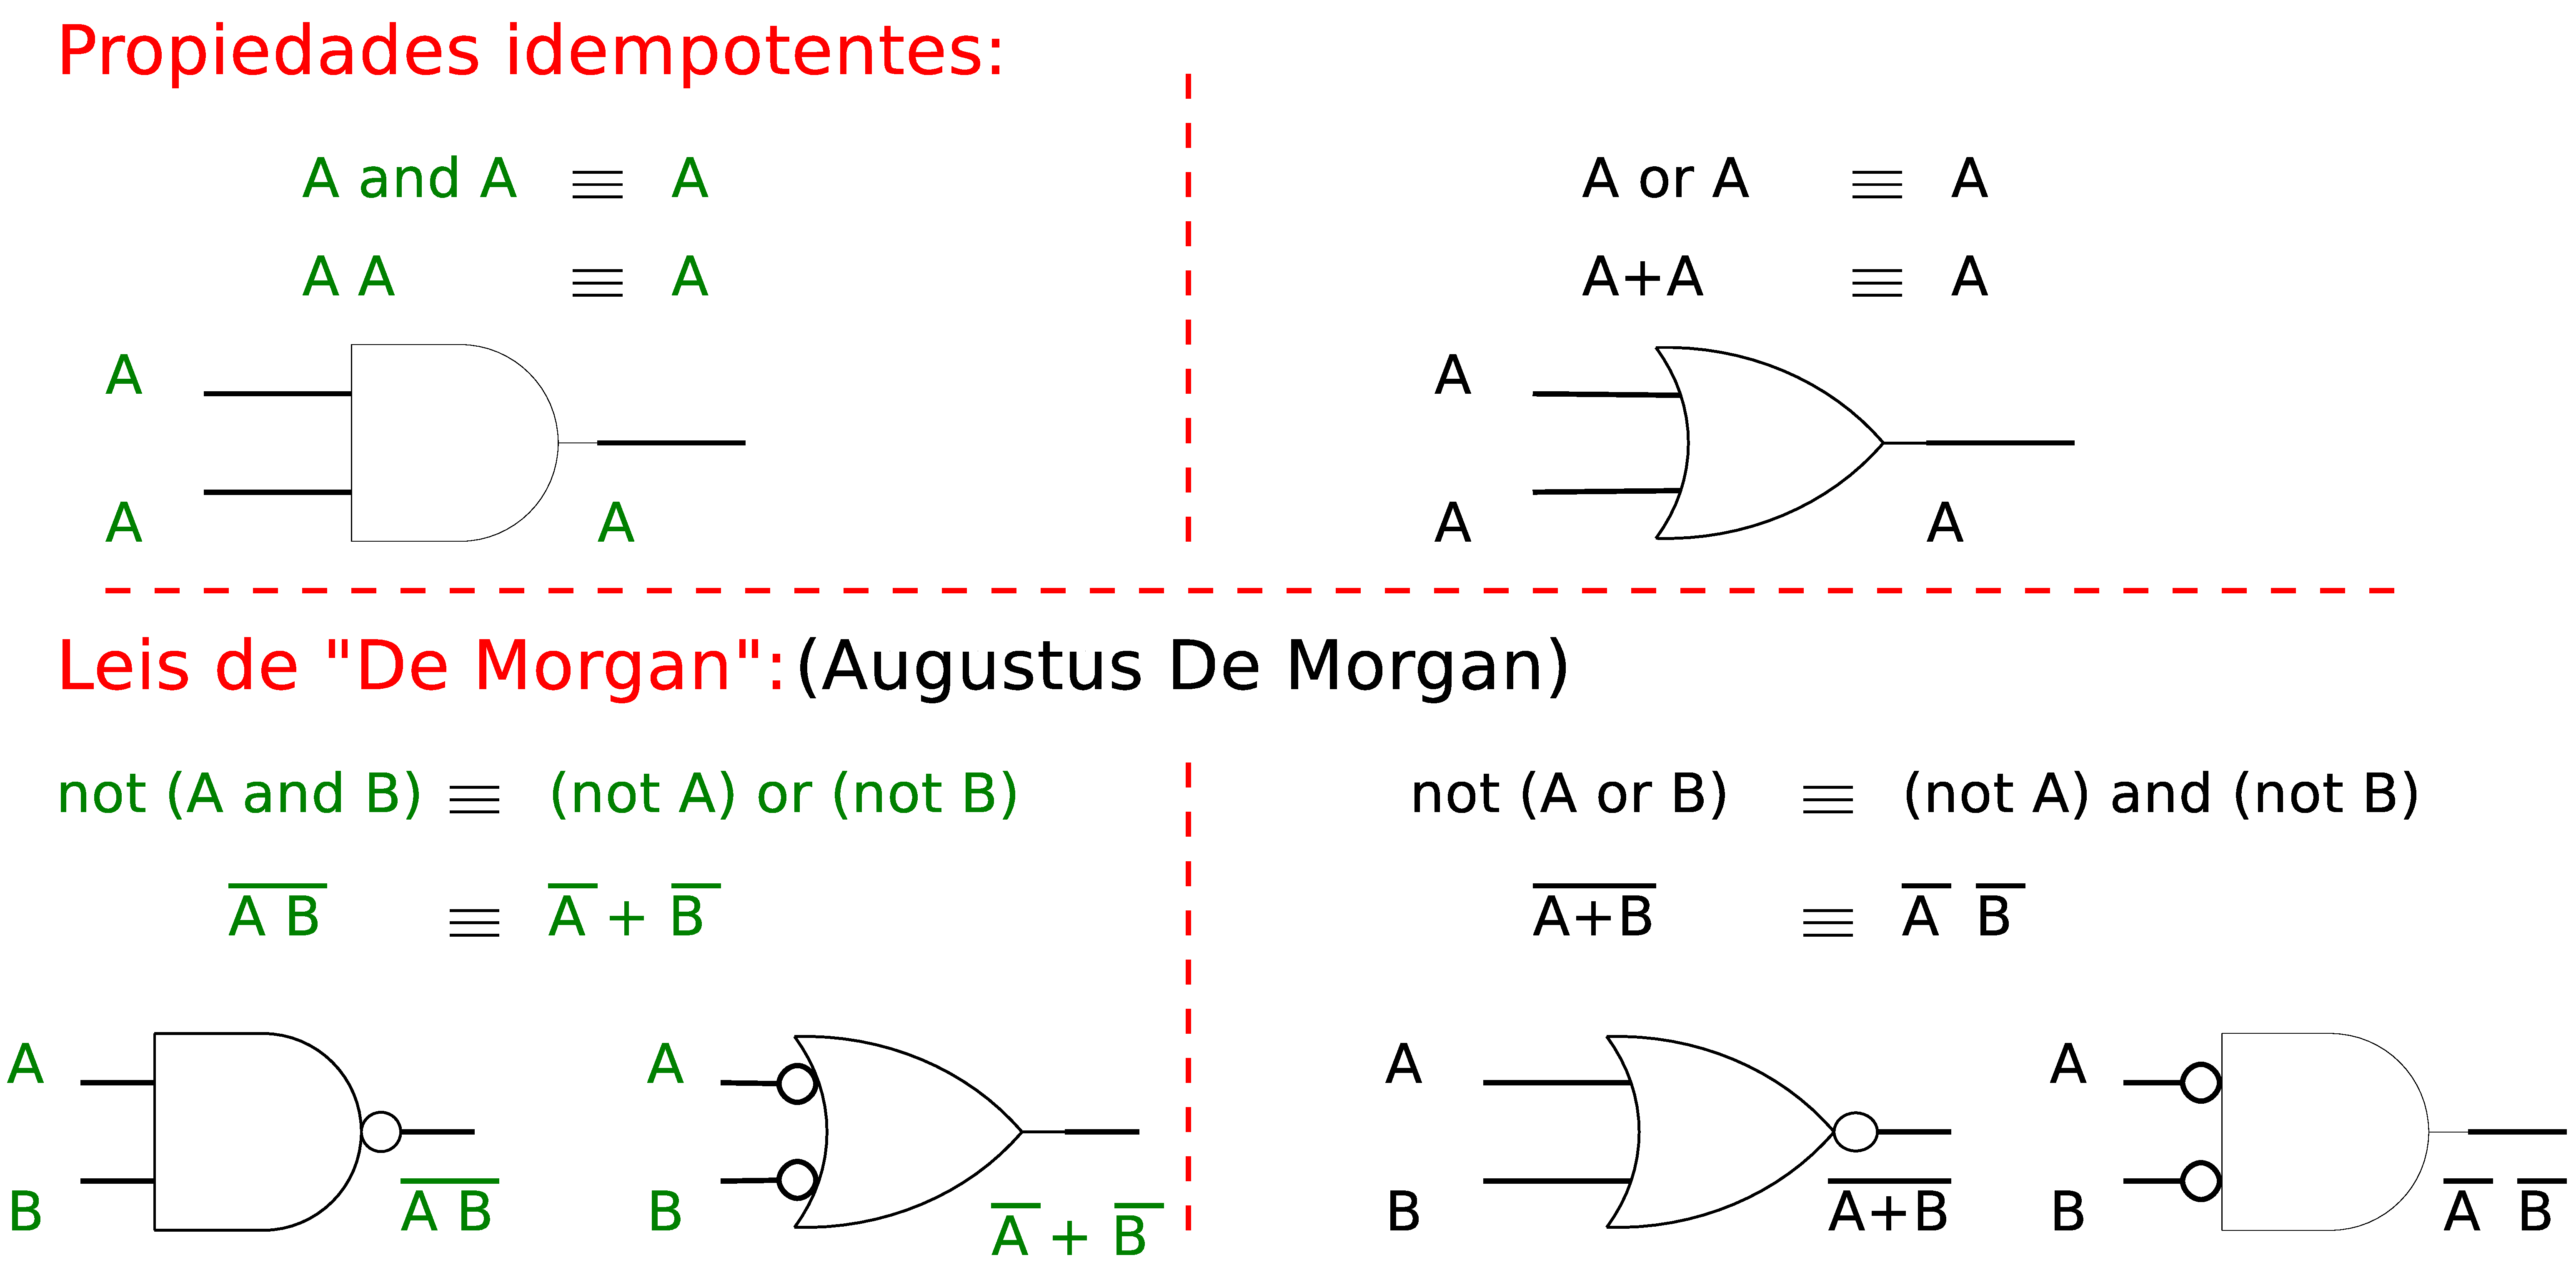
\includegraphics[width=0.99\textwidth]{images/idempotente.eps}
\end{center} 
\end{frame}

%%%%%%%%%%%%%%%%%%%%%%%%%%%%%%%%%%%%%%%%%%%%%%%%%%%%%%%%%%%%%%%%%%%%%%%%%%%%%%%%
\begin{frame}{Projetando um circuito lógico}
\begin{center}
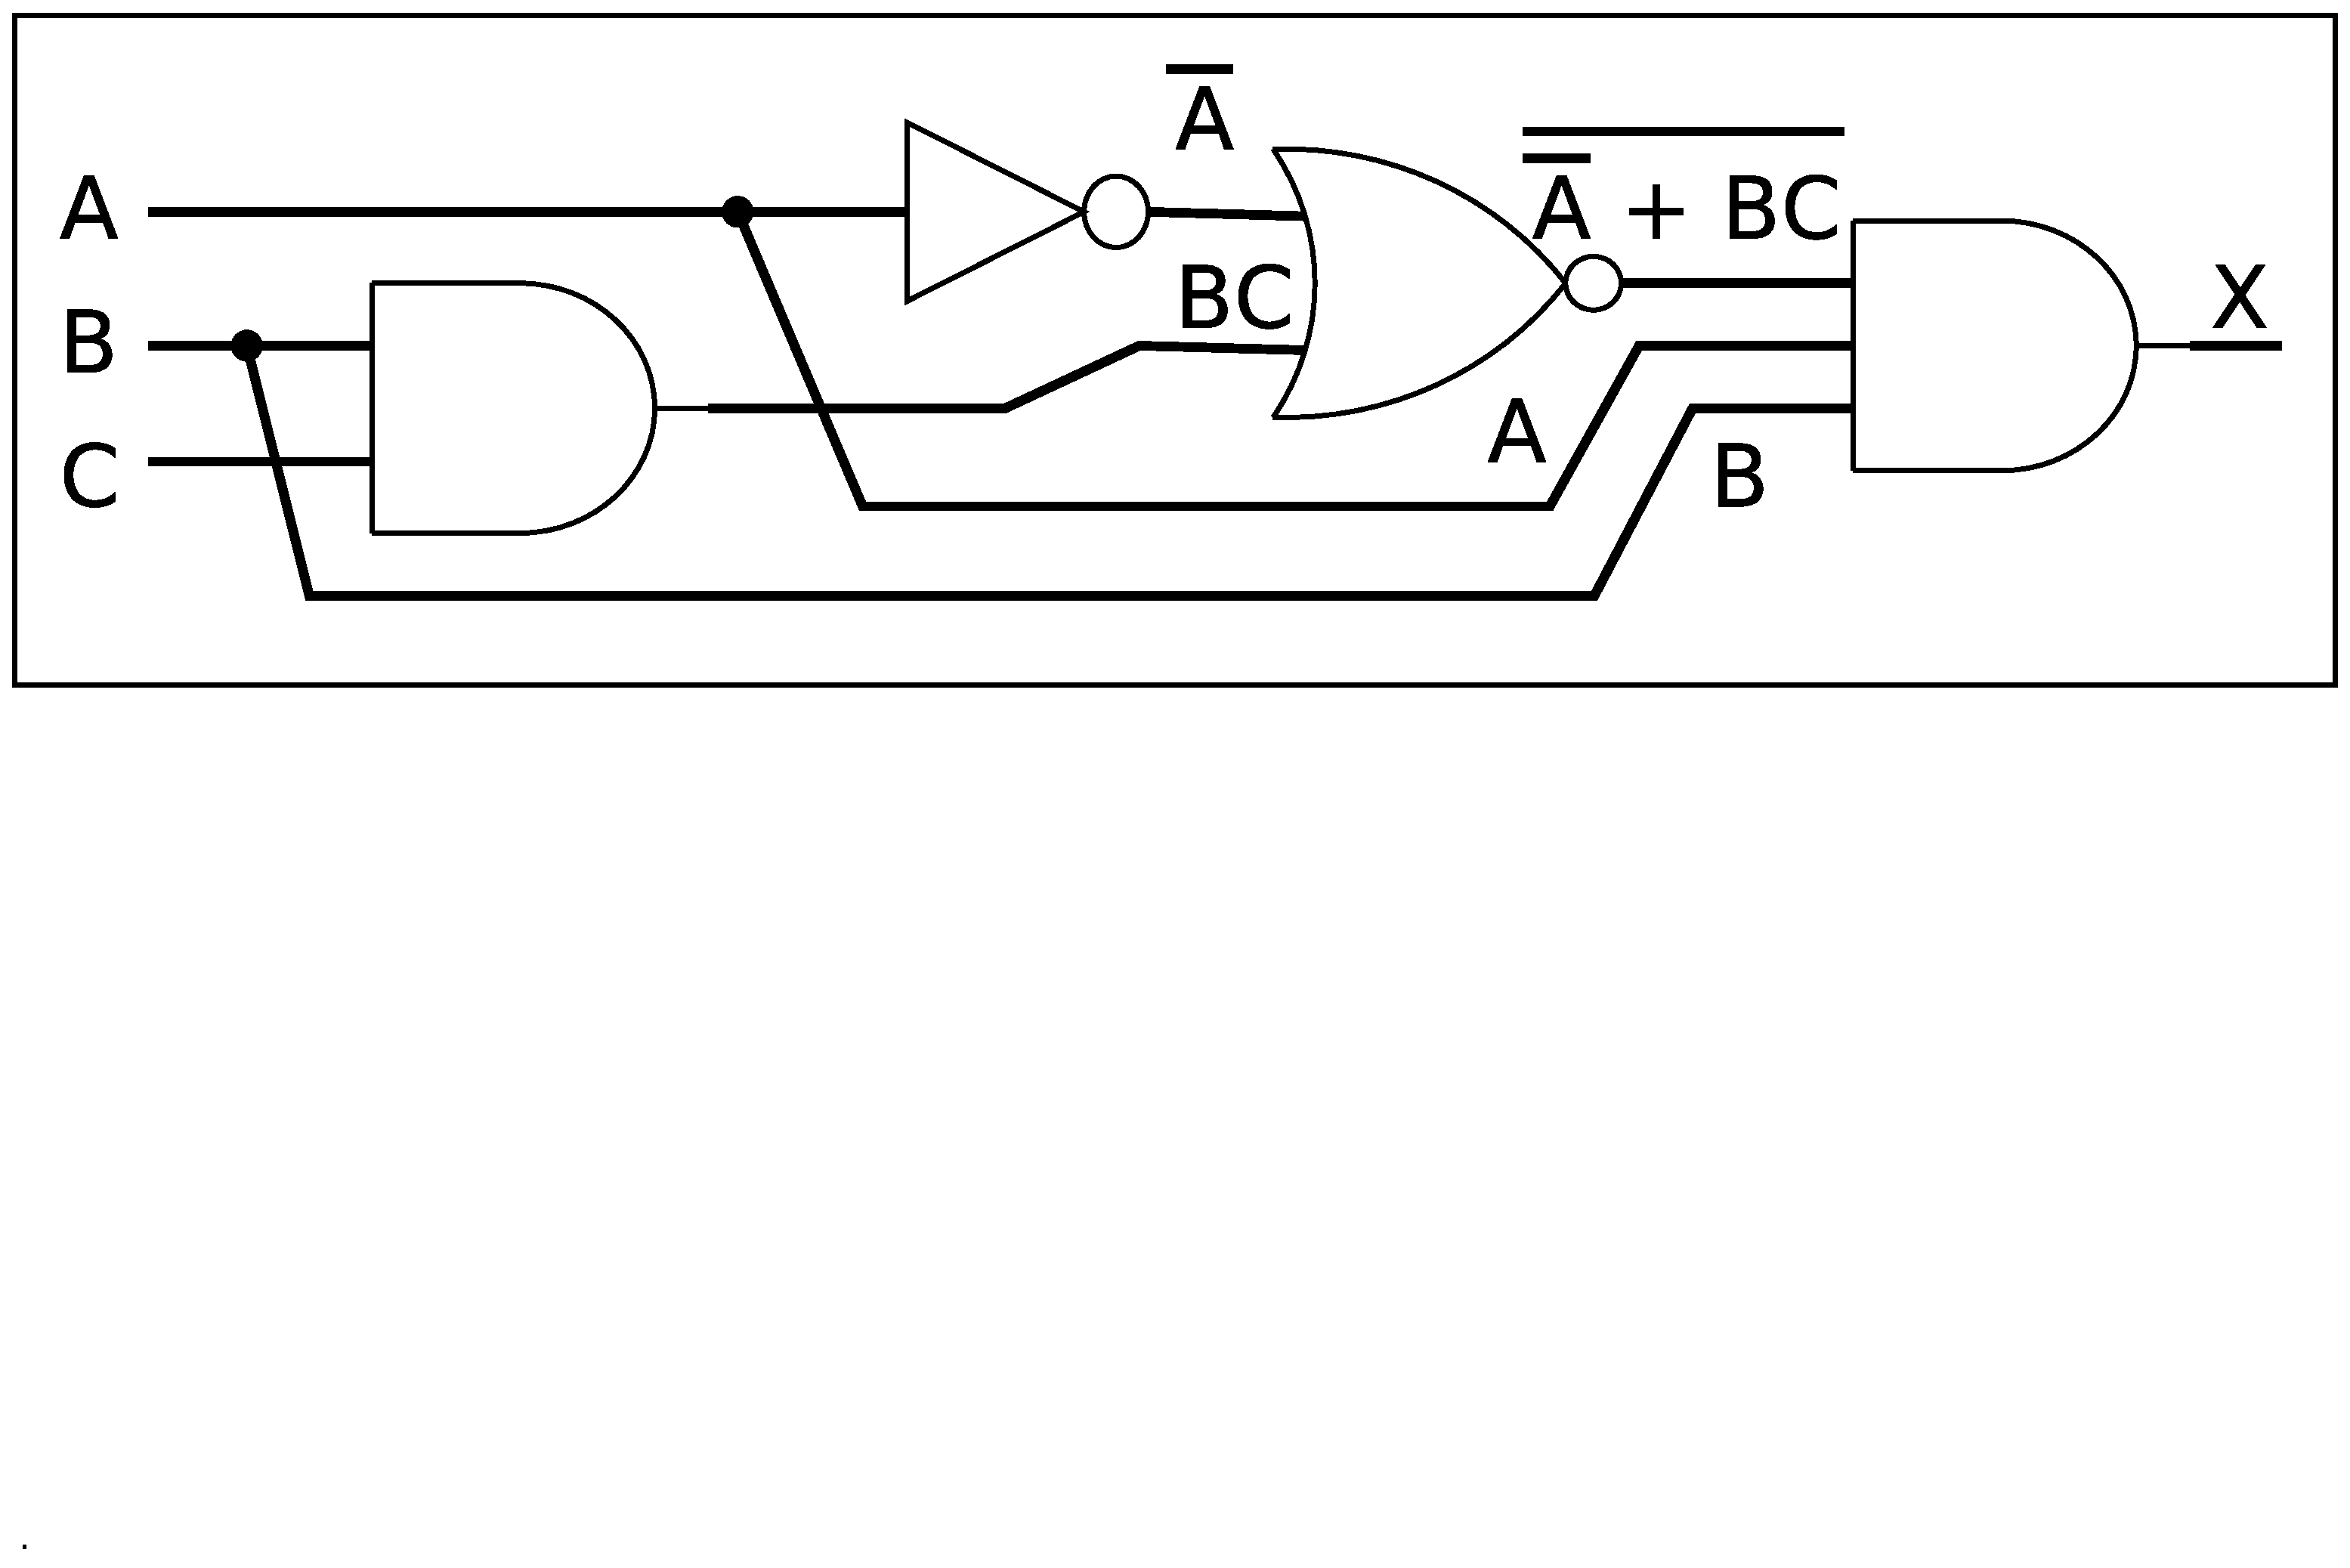
\includegraphics[width=0.99\textwidth]{images/simplifica1a.eps}
\end{center} 
\end{frame}

%%%%%%%%%%%%%%%%%%%%%%%%%%%%%%%%%%%%%%%%%%%%%%%%%%%%%%%%%%%%%%%%%%%%%%%%%%%%%%%%
\begin{frame}{Projetando um circuito lógico}
\begin{center}
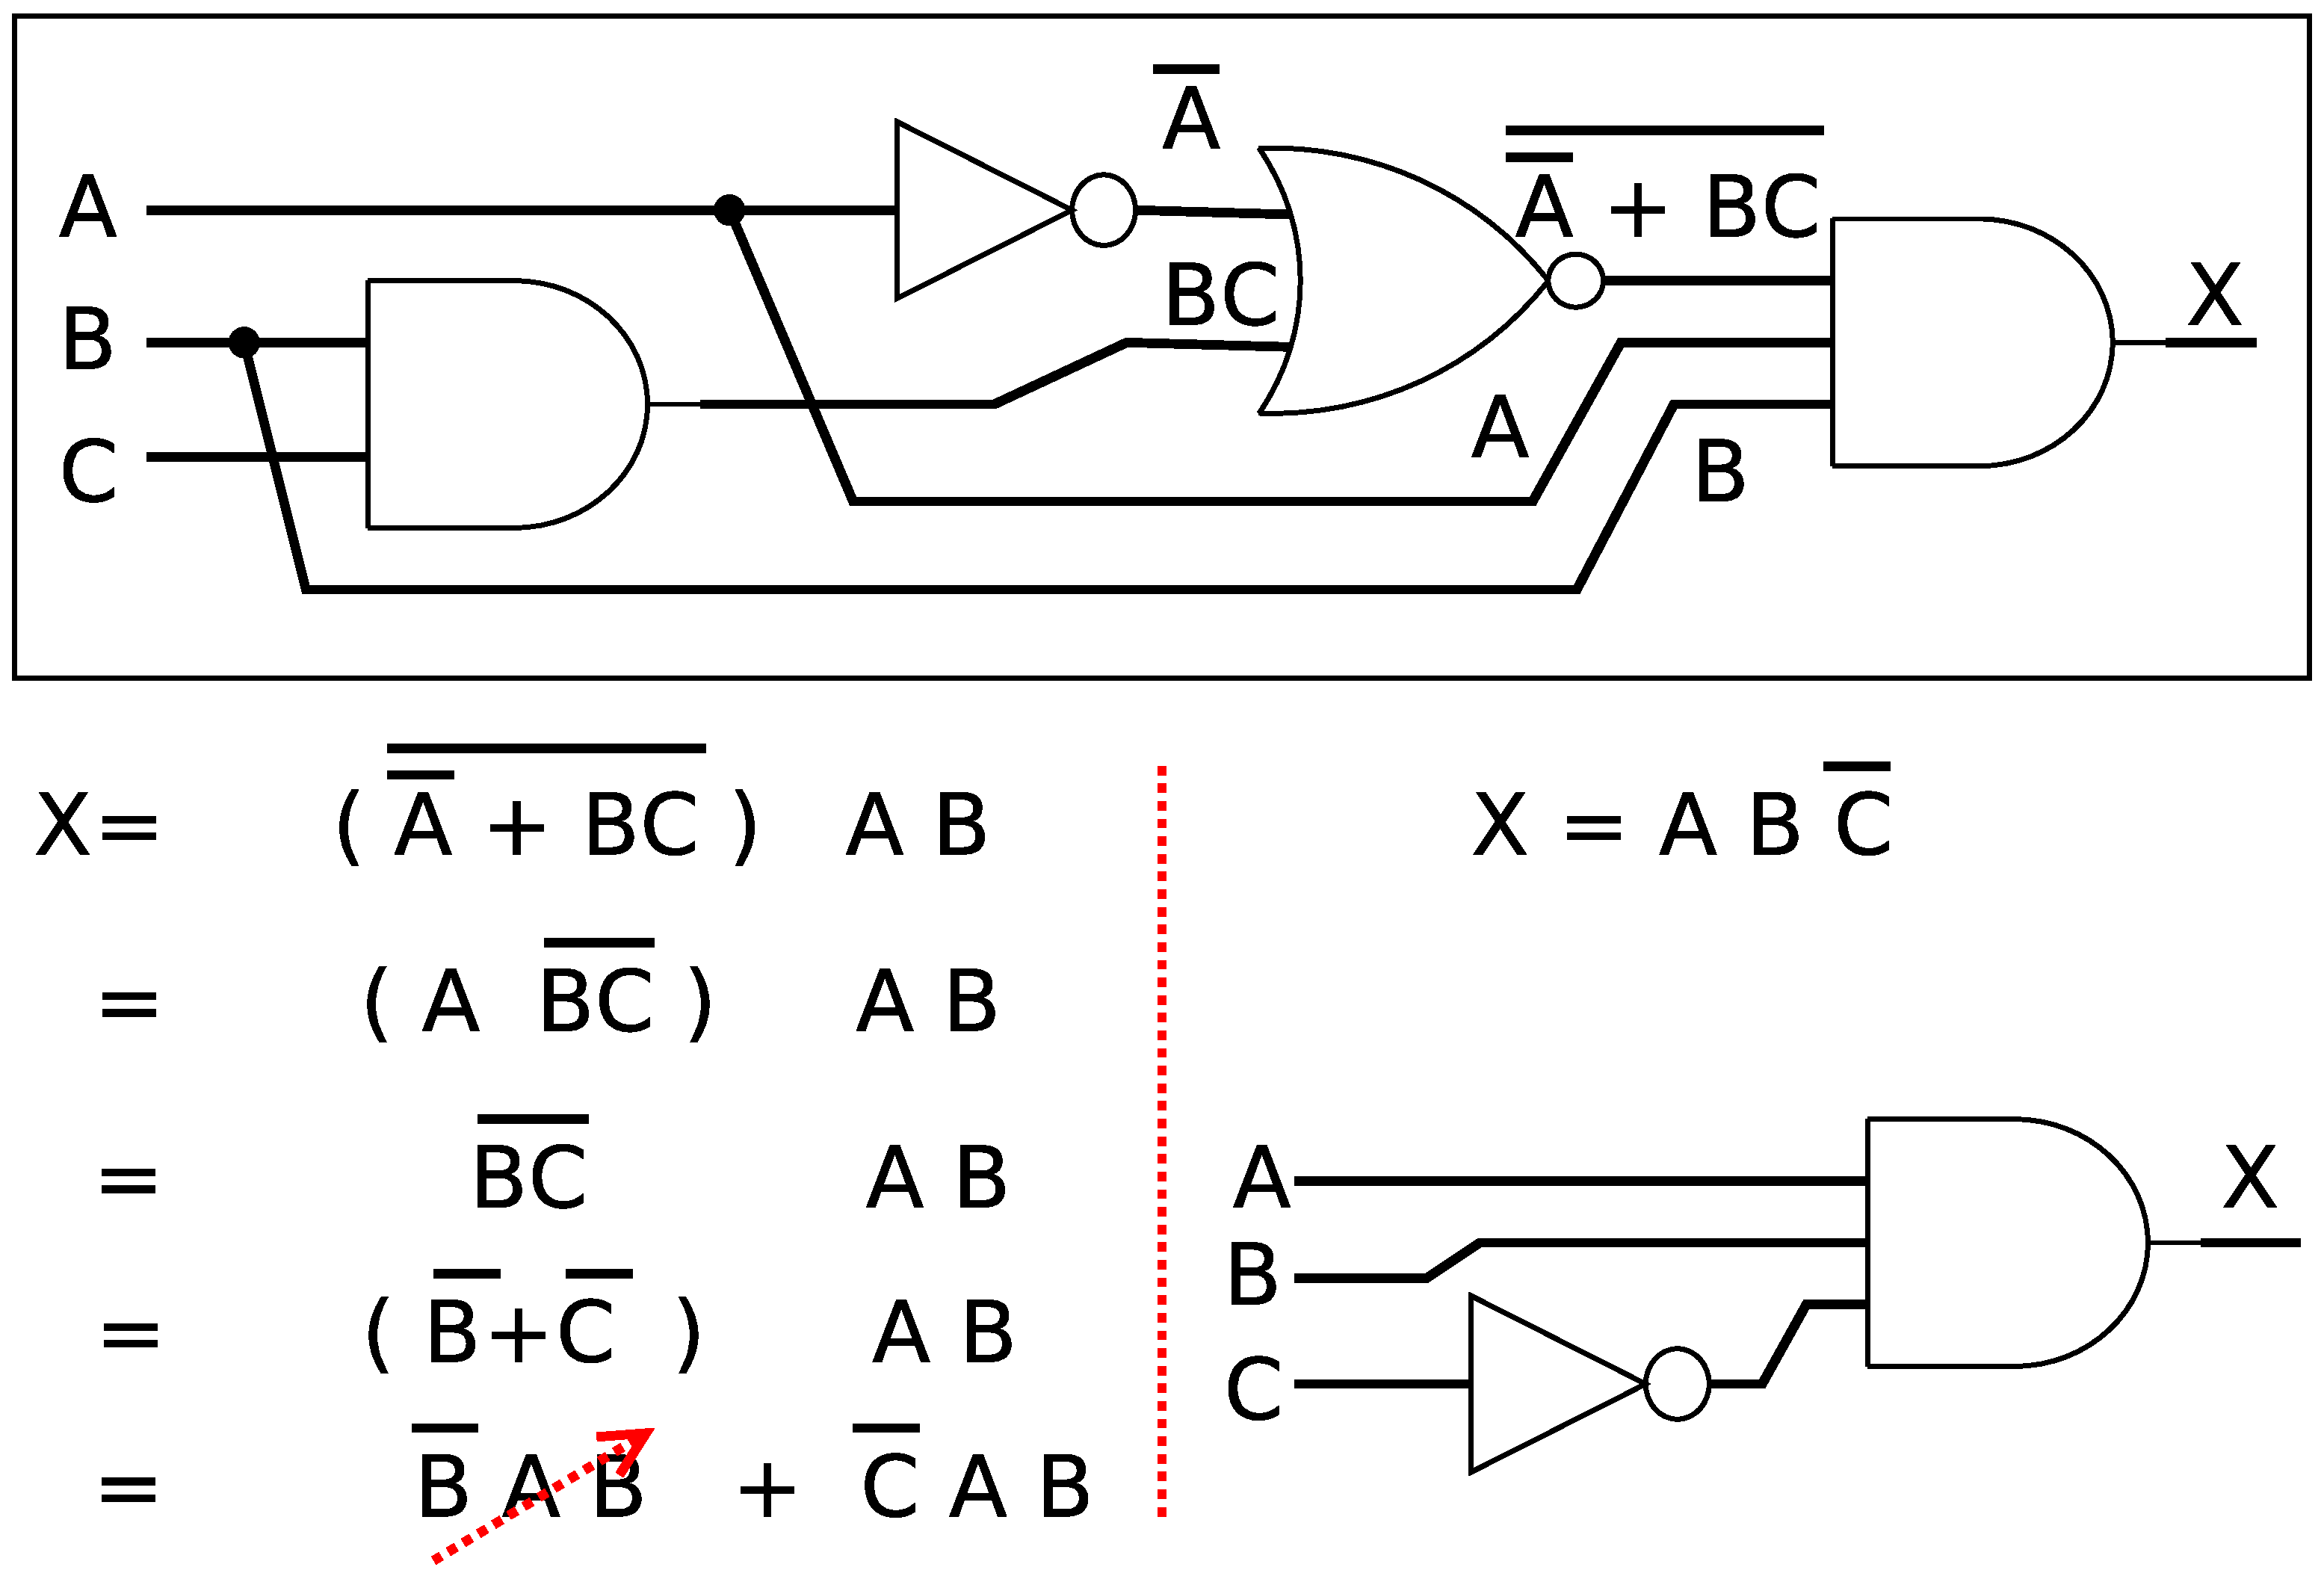
\includegraphics[width=0.99\textwidth]{images/simplifica1.eps}
\end{center} 
\end{frame}

%%%%%%%%%%%%%%%%%%%%%%%%%%%%%%%%%%%%%%%%%%%%%%%%%%%%%%%%%%%%%%%%%%%%%%%%%%%%%%%%
\begin{frame}{Projetando um circuito lógico}
\begin{center}
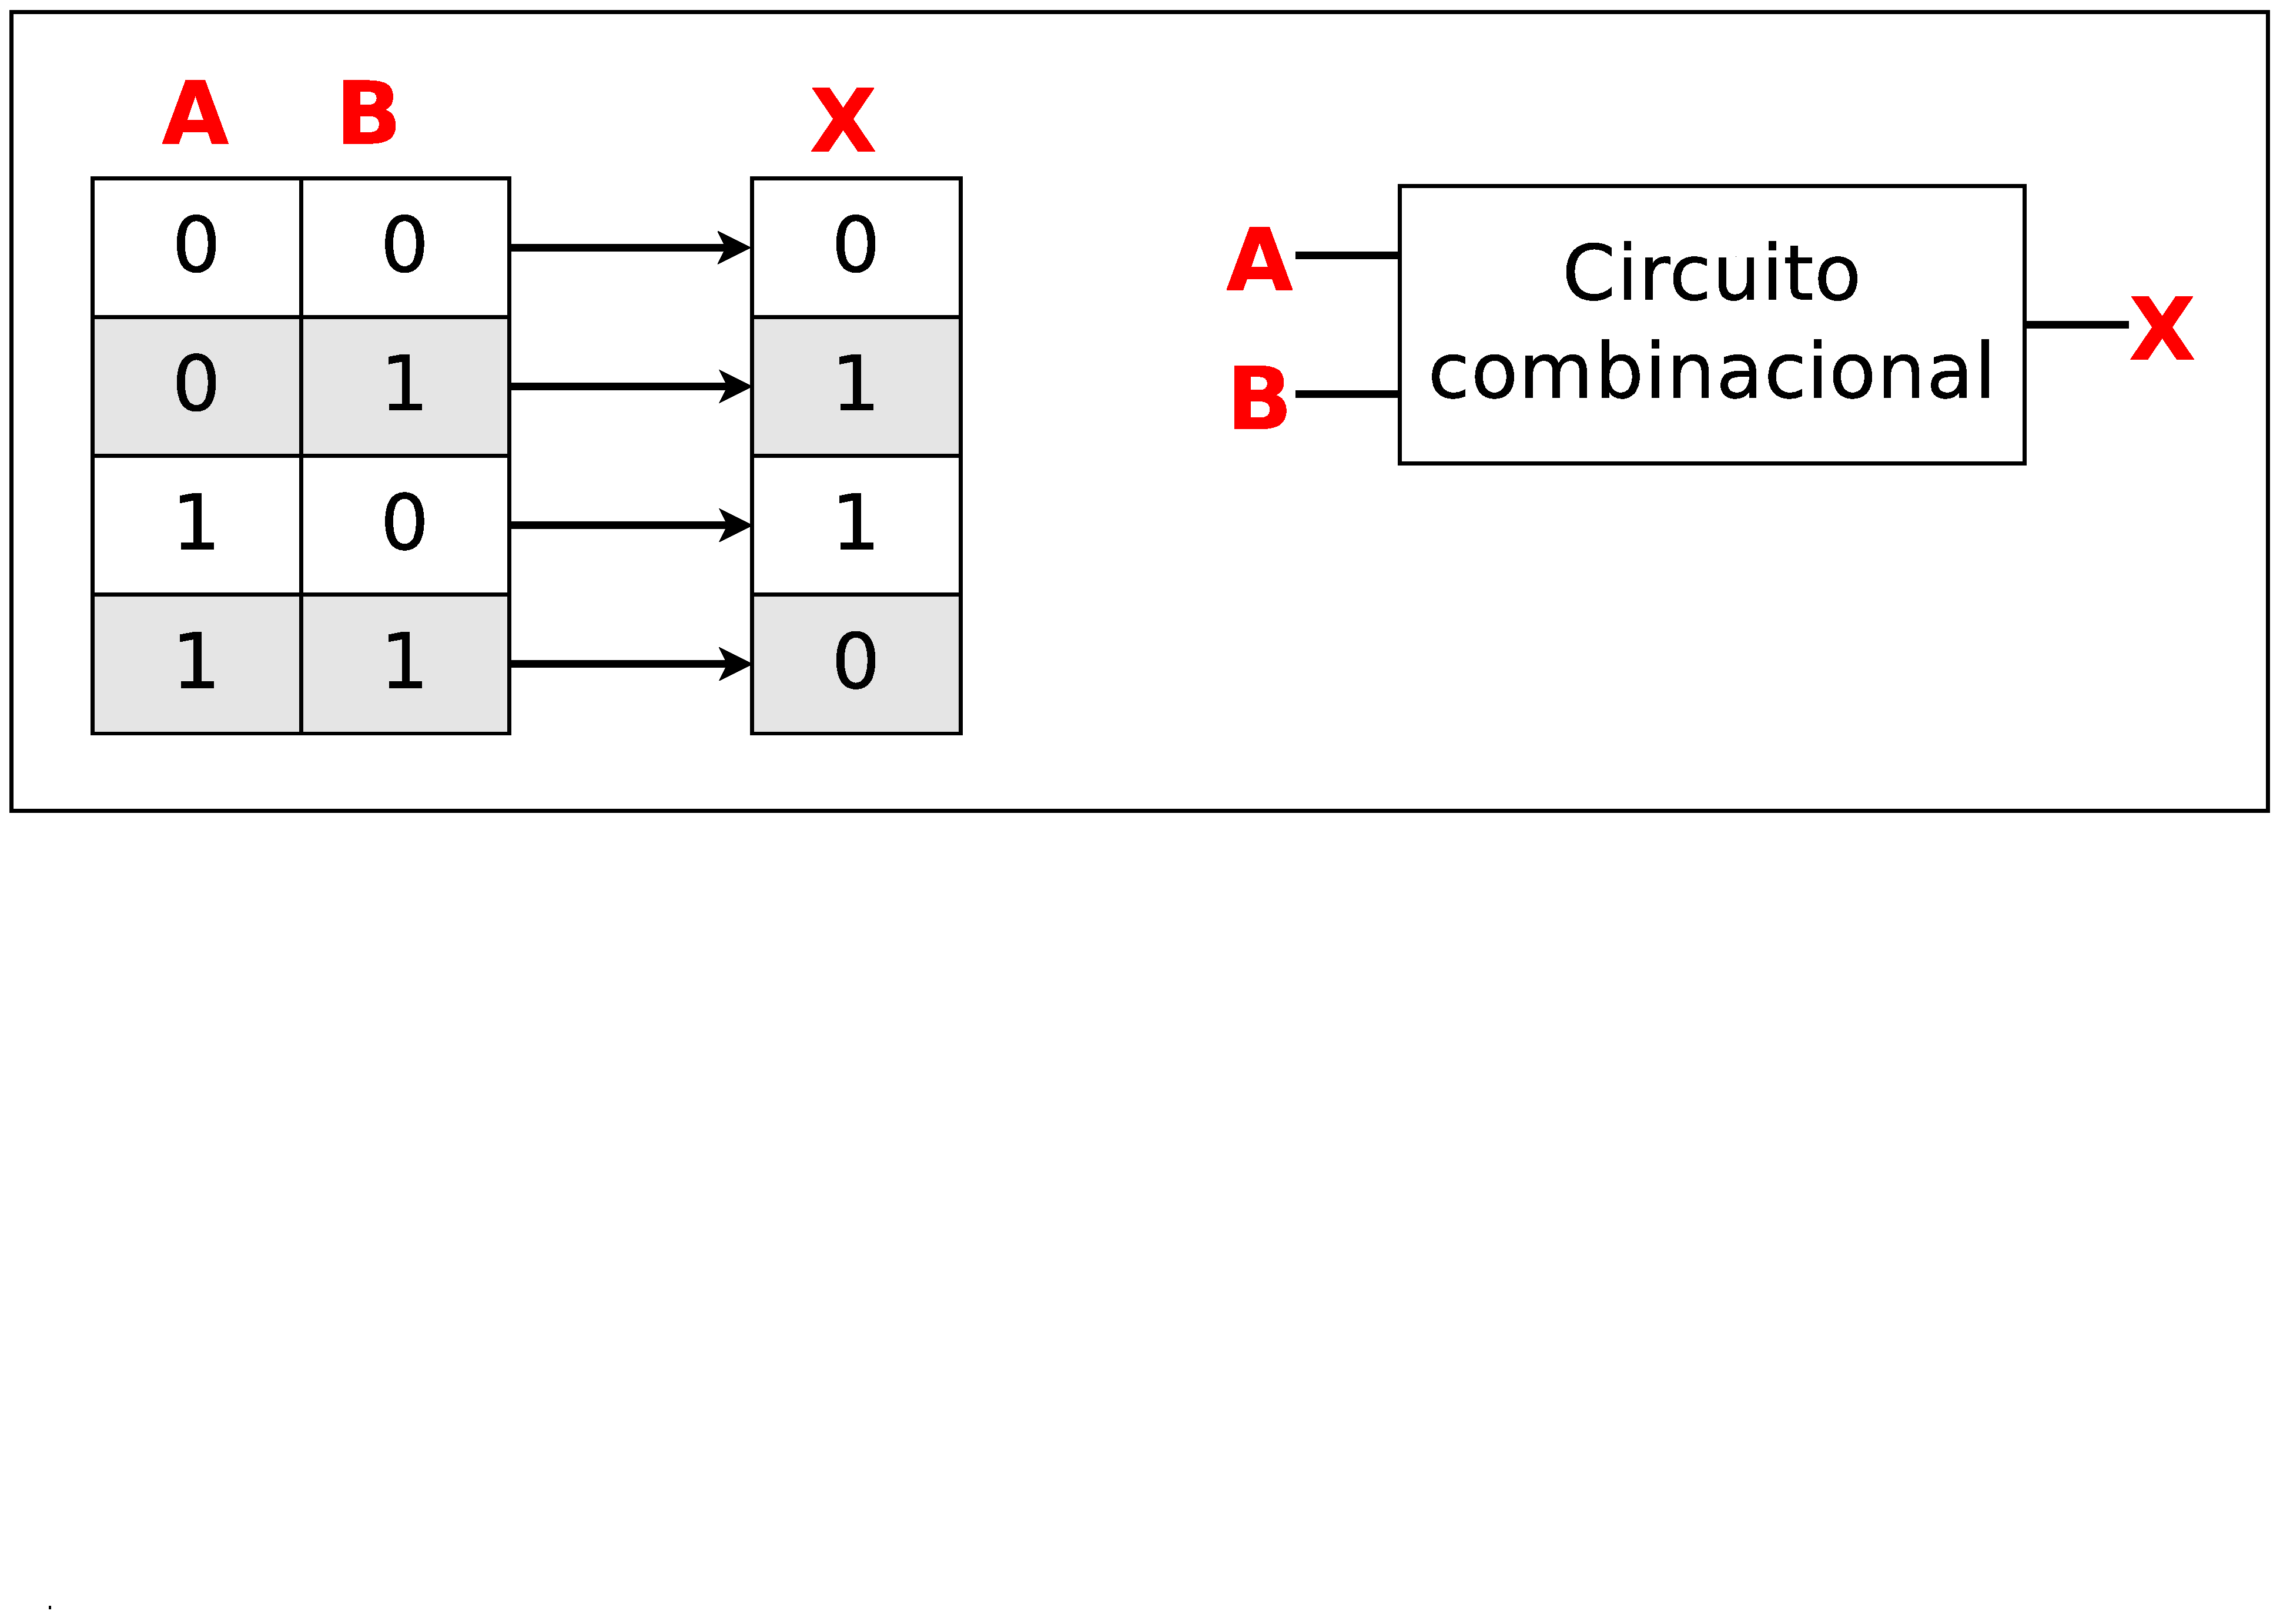
\includegraphics[width=0.7\textwidth]{images/circuito1.eps}
\end{center} 
\end{frame}

%%%%%%%%%%%%%%%%%%%%%%%%%%%%%%%%%%%%%%%%%%%%%%%%%%%%%%%%%%%%%%%%%%%%%%%%%%%%%%%%
\begin{frame}{Projetando um circuito lógico}
\begin{center}
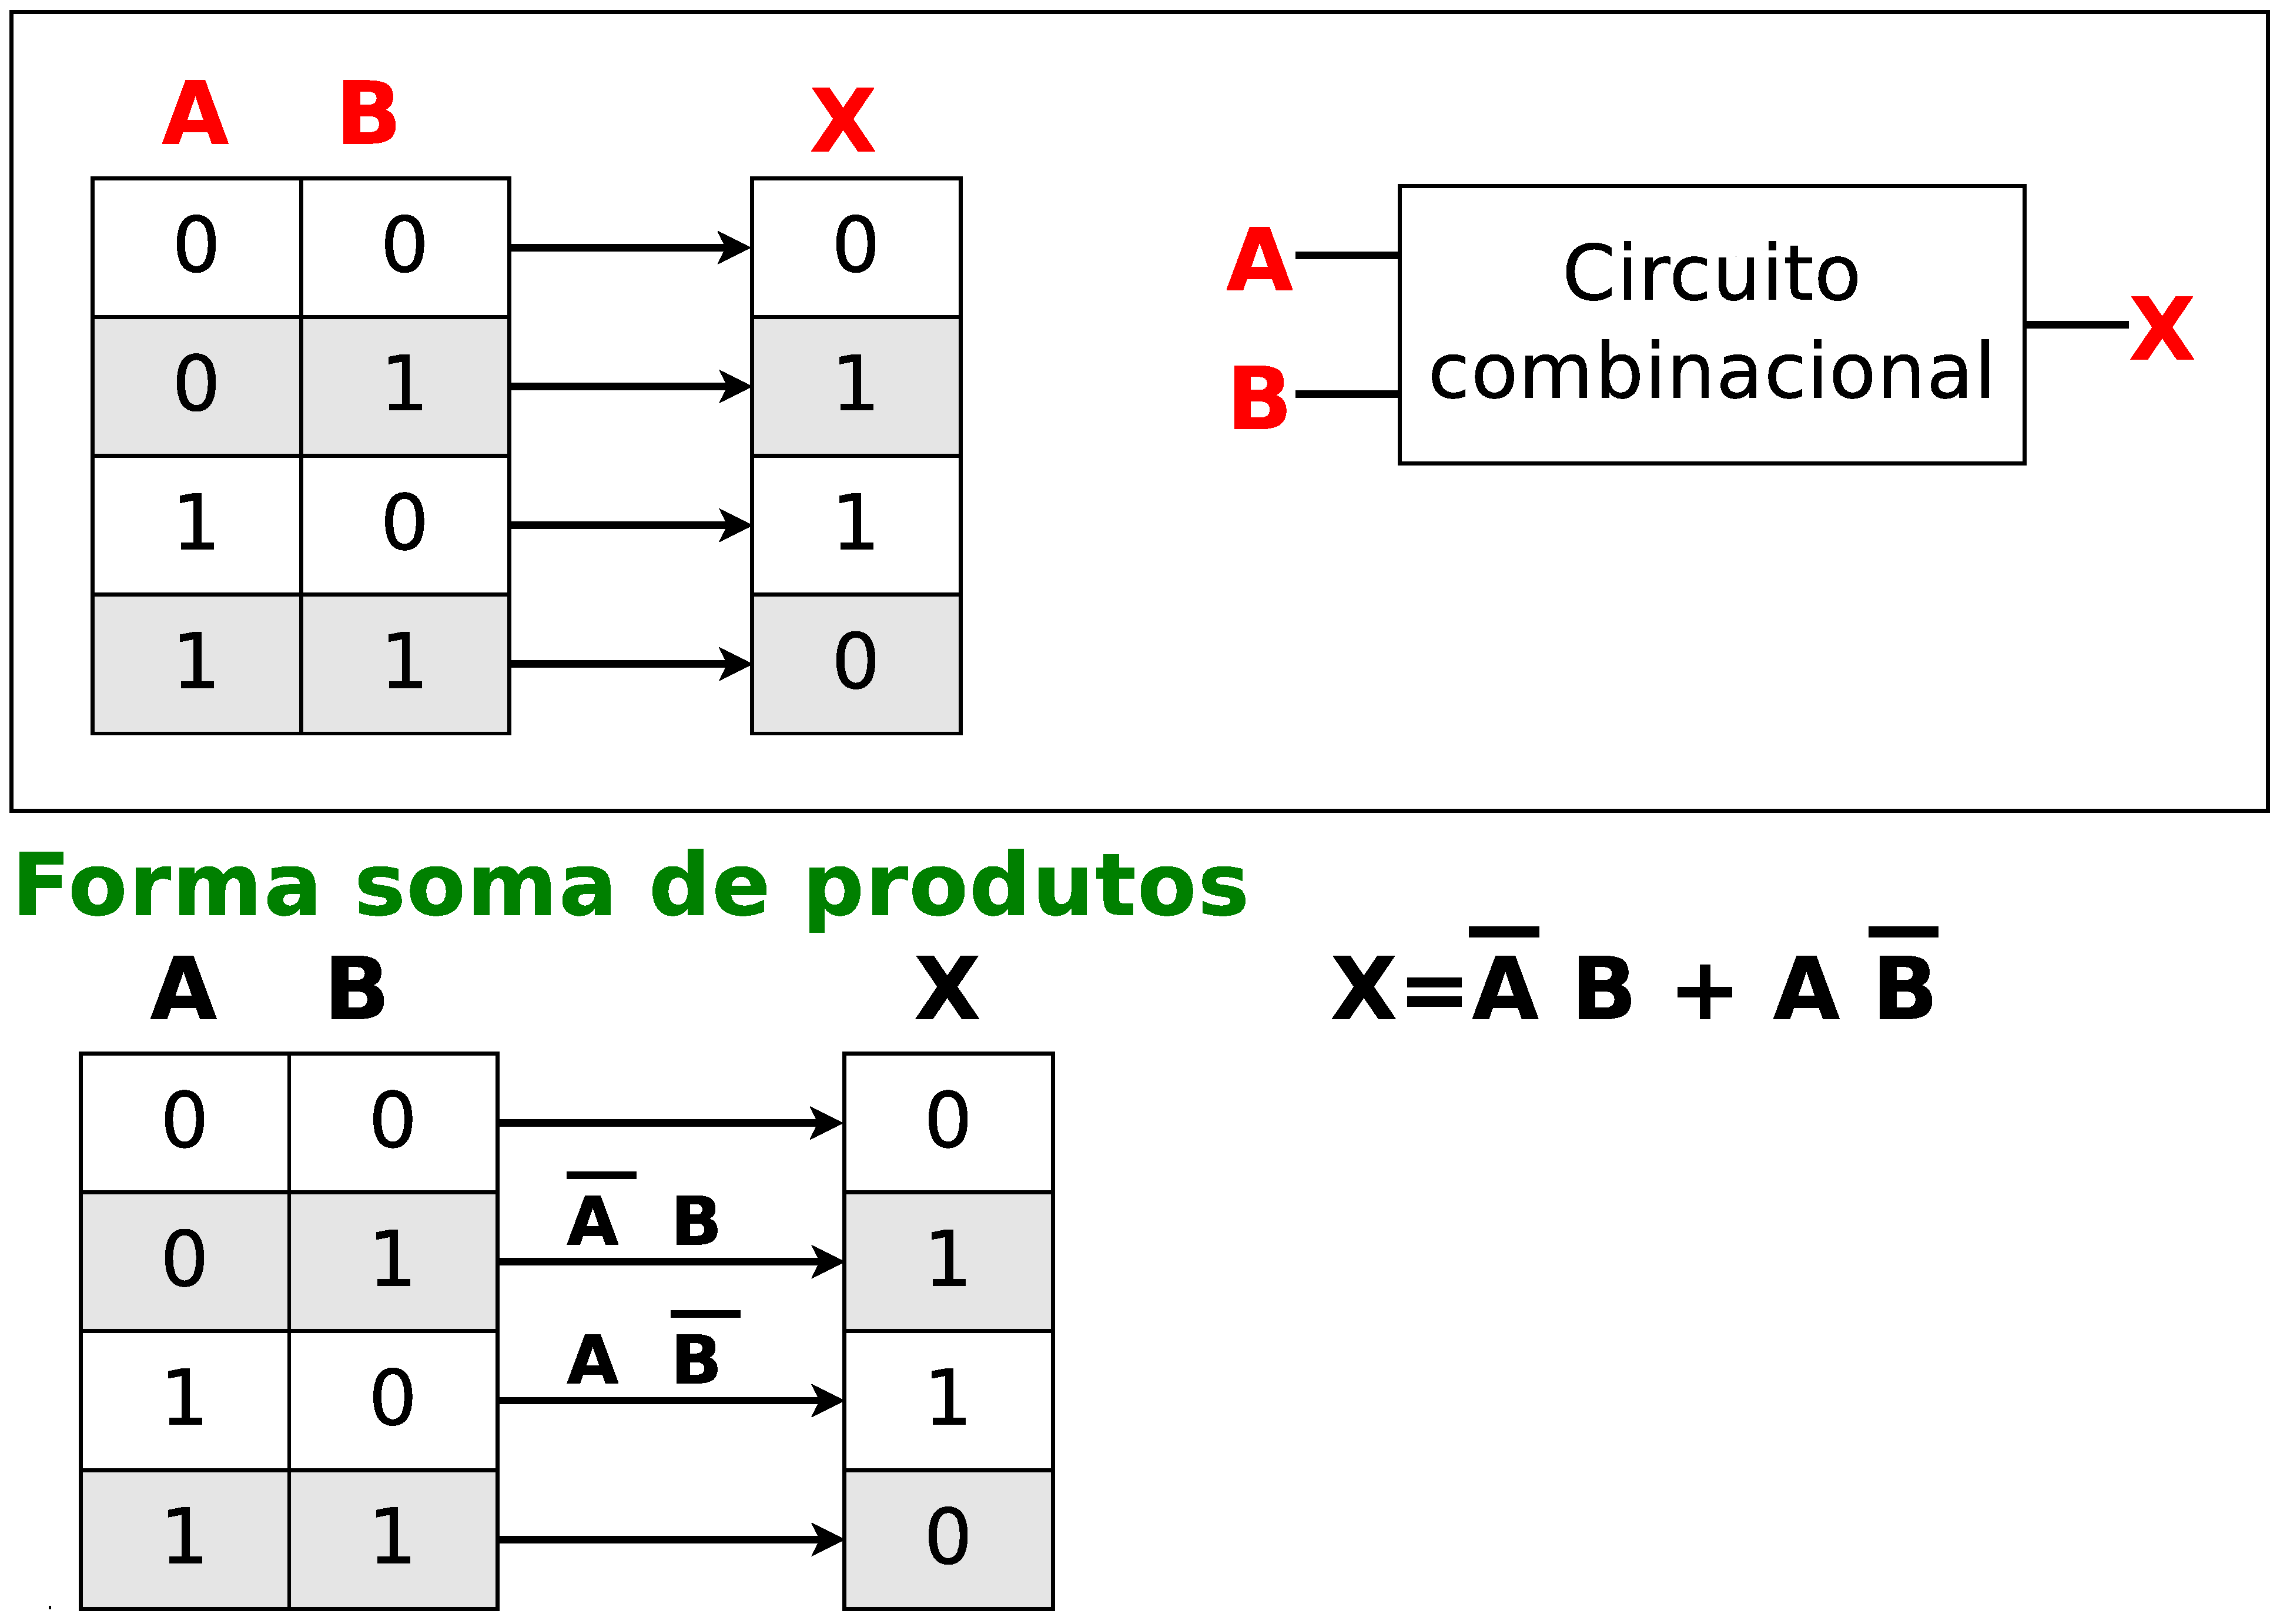
\includegraphics[width=0.7\textwidth]{images/circuito1a.eps}
\end{center} 
\end{frame}

%%%%%%%%%%%%%%%%%%%%%%%%%%%%%%%%%%%%%%%%%%%%%%%%%%%%%%%%%%%%%%%%%%%%%%%%%%%%%%%%
\begin{frame}{Projetando um circuito lógico}
\begin{center}
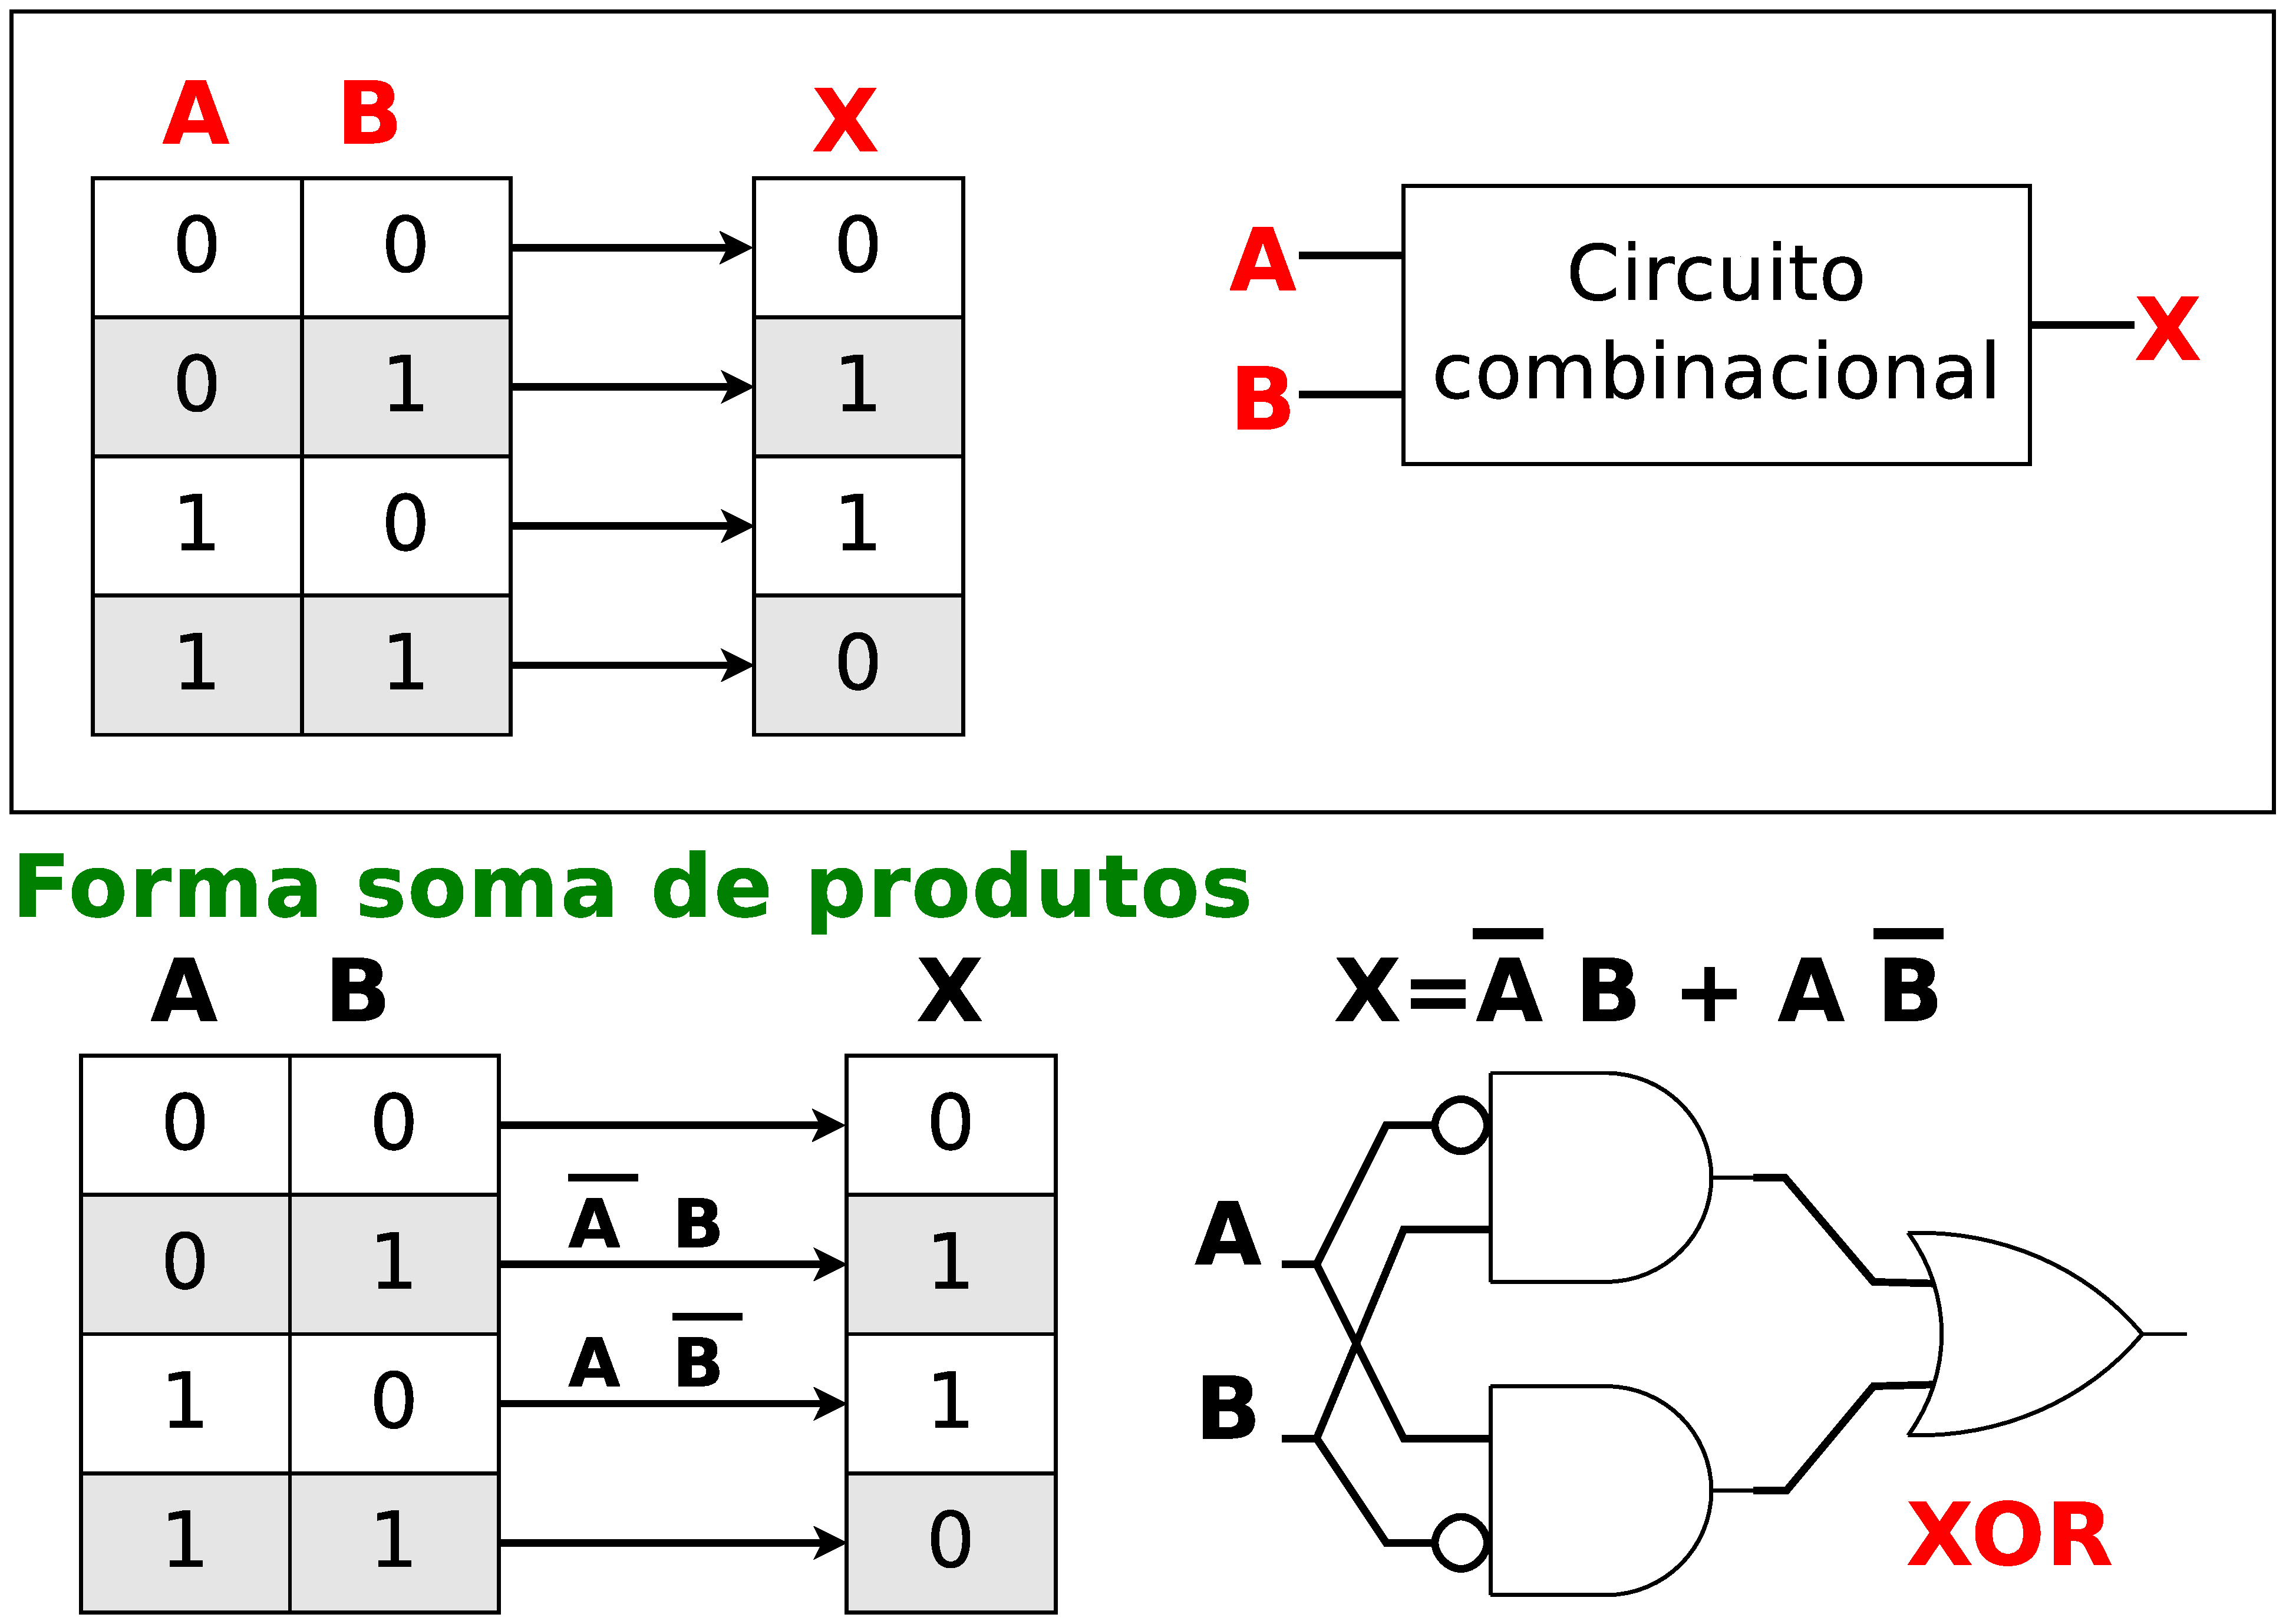
\includegraphics[width=0.7\textwidth]{images/circuito1b.eps}
\end{center} 
\end{frame}

%siplificar : https://www.youtube.com/watch?v=8ST9tLxppxI


%%%%%%%%%%%%%%%%%%%%%%%%%%%%%%%%%%%%%%%%%%%%%%%%%%%%%%%%%%%%%%%%%%%%%%%%%%%%%%%%
%Mapa de Karnaugh : https://www.youtube.com/watch?v=SI8MkT-HTL8
\begin{frame}{Projetando: Mapa de Karnaugh \cite{tocci2003sistemas}}
\begin{center}
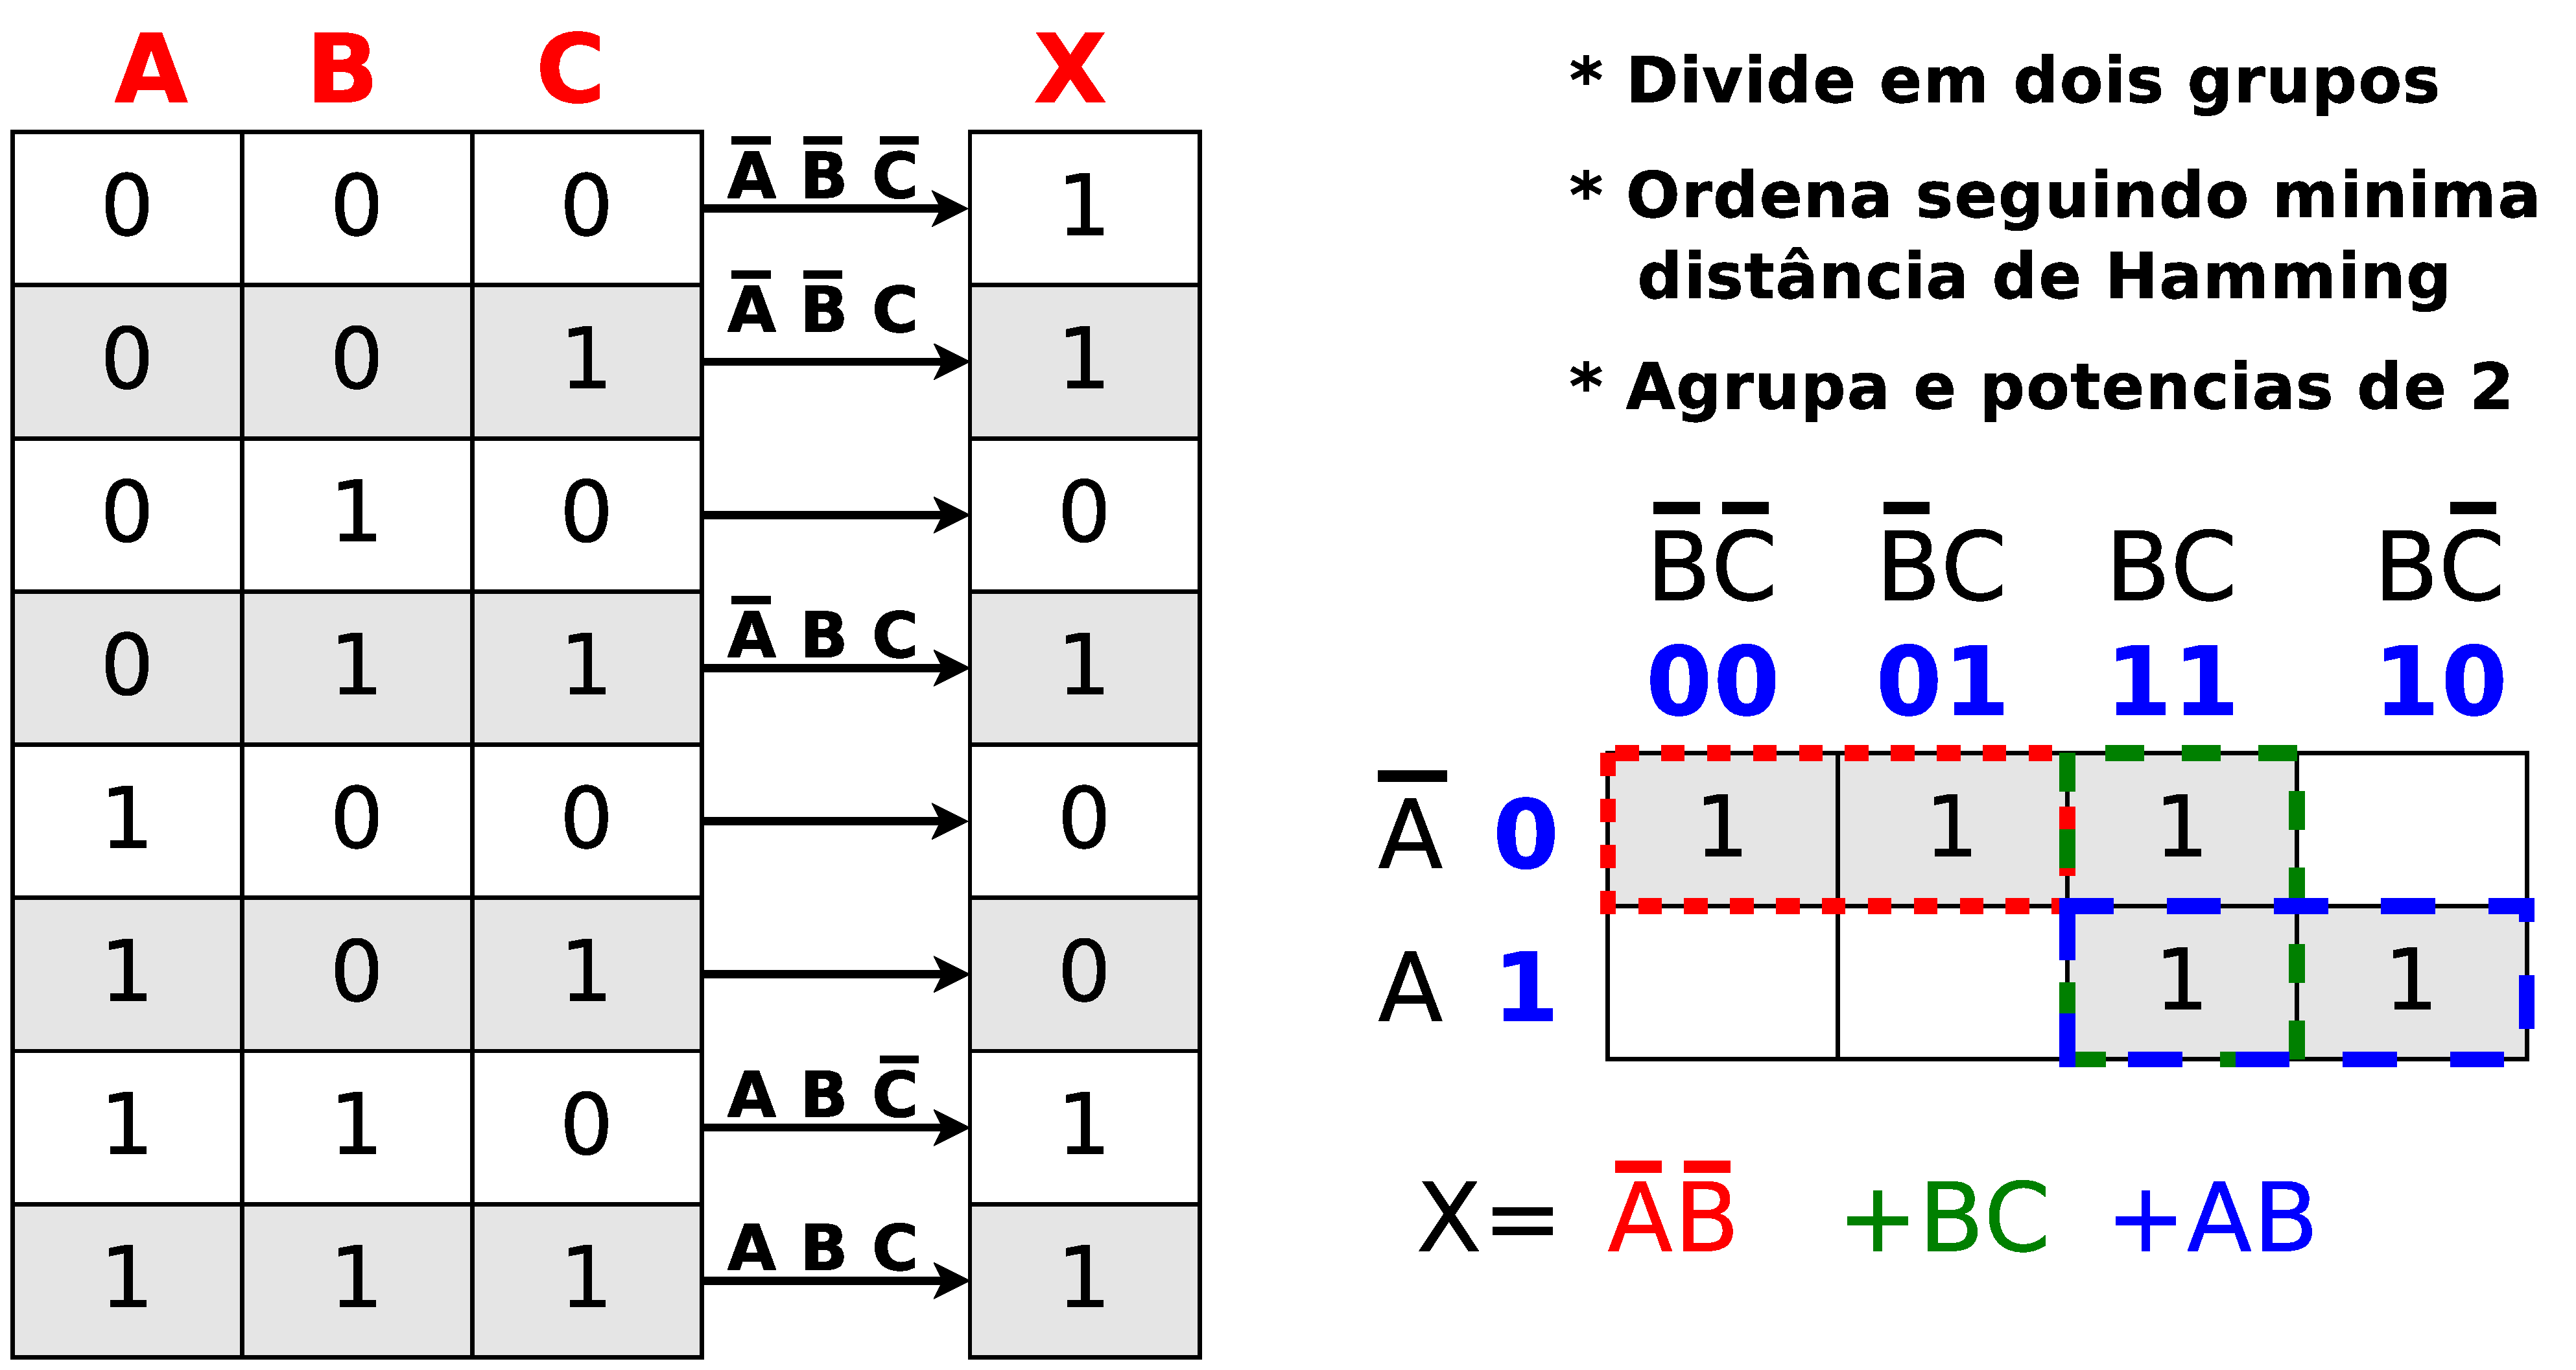
\includegraphics[width=0.99\textwidth]{images/circuito3.eps}
\end{center} 
\end{frame}

%%%%%%%%%%%%%%%%%%%%%%%%%%%%%%%%%%%%%%%%%%%%%%%%%%%%%%%%%%%%%%%%%%%%%%%%%%%%%%%%
\begin{frame}{Projetando: Mapa de Karnaugh}
\begin{center}
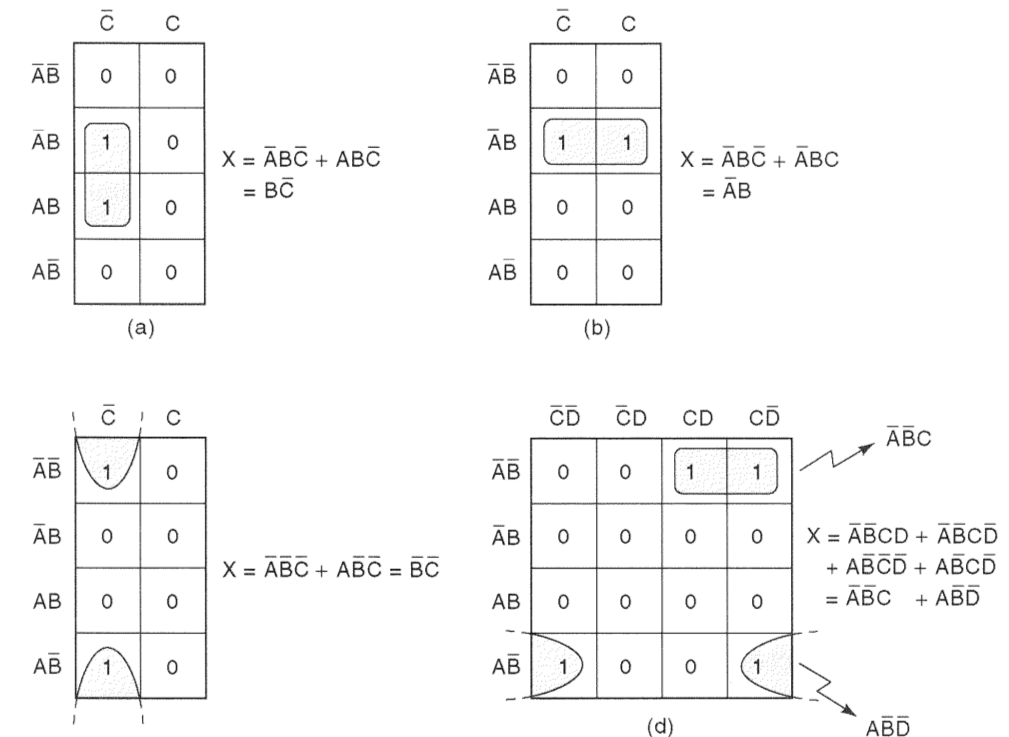
\includegraphics[width=0.8\textwidth]{images/mapak2.eps}
\end{center} 
\end{frame}

%%%%%%%%%%%%%%%%%%%%%%%%%%%%%%%%%%%%%%%%%%%%%%%%%%%%%%%%%%%%%%%%%%%%%%%%%%%%%%%%
\begin{frame}{Projetando: Mapa de Karnaugh}
\begin{center}
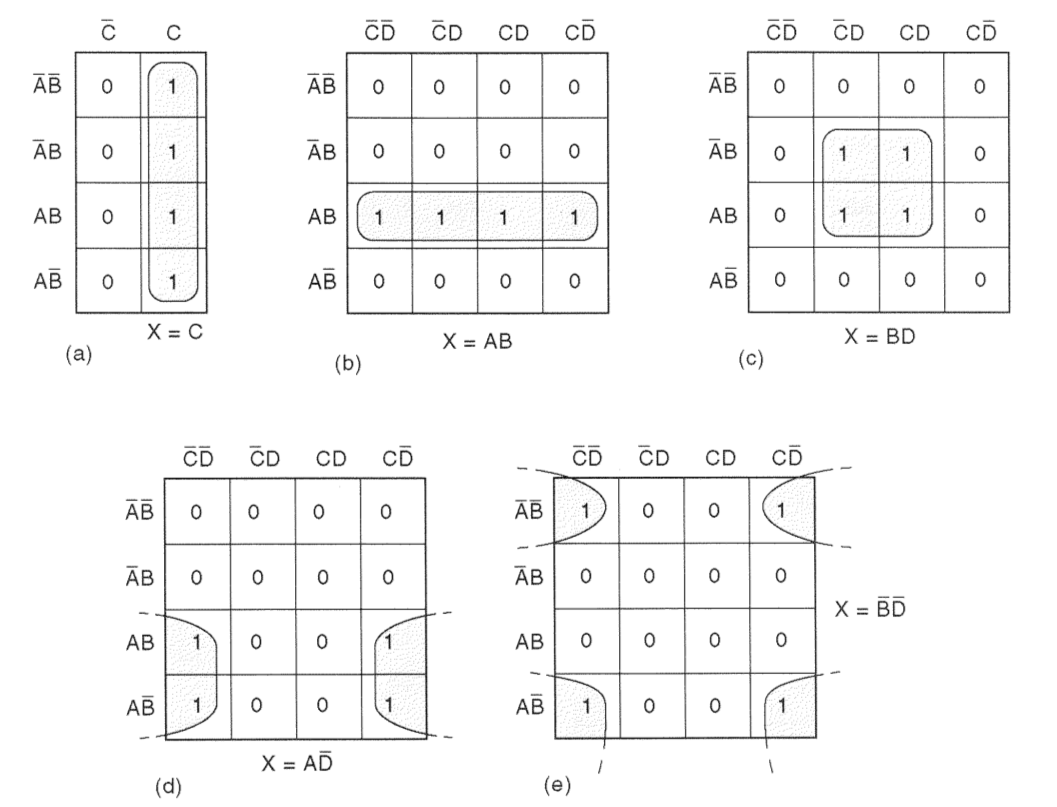
\includegraphics[width=0.8\textwidth]{images/mapak4.eps}
\end{center} 
\end{frame}

%%%%%%%%%%%%%%%%%%%%%%%%%%%%%%%%%%%%%%%%%%%%%%%%%%%%%%%%%%%%%%%%%%%%%%%%%%%%%%%%
\begin{frame}[allowframebreaks]
        \frametitle{References}
        \bibliographystyle{plain}
\bibliography{combinacional}
\end{frame}



\end{document}
